\documentclass[british,titlepage]{ntnuthesis}
\usepackage{graphicx}
\usepackage{array}
\usepackage{biblatex}
\usepackage{subcaption}
\usepackage{float}
\usepackage{longtable}
\usepackage{listings}
\usepackage{xcolor}
\usepackage{multirow}
\lstset{language=Python,
    basicstyle=\ttfamily,
    keywordstyle=\color{blue}\ttfamily,
    stringstyle=\color{red}\ttfamily,
    commentstyle=\color{green}\ttfamily,
    morecomment=[l][\color{magenta}]{\#},
    showstringspaces=false,
    breaklines=true,
    frame=tb
}


\title{Sensitive Information Exposed By The Use Of Robot Vacuum Cleaners In Smart Homes }
\shorttitle{Sensitive Information Exposed By The Use Of Robot Vacuum Cleaners In Smart Homes}
\author{Benjamin Andreas Ulsmåg}
\shortauthor{Benjamin A. U.}
\date{CC-BY \ntnuthesisdate}

\addbibresource{thesis.bib}



% From https://www.overleaf.com/learn/latex/Glossaries

\makeglossaries % Prepare for adding glossary entries


\newglossaryentry{latex}
{
        name=latex,
        description={Is a mark up language specially suited for
scientific documents}
}

\newglossaryentry{bibliography}
{
        name=bibliography,
        plural=bibliographies,
        description={A list of the books referred to in a scholarly work,
typically printed as an appendix}
}

\newglossaryentry{maths}
{
    name=mathematics,
    description={Mathematics is what mathematicians do}
}


% --------------------
% ----- Acronyms -----
% --------------------

\newacronym{phd}{PhD}{philosophiae doctor}
\newacronym{CoPCSE}{CoPCSE@NTNU}{Community of Practice in Computer ScienceEducation at NTNU}
\newacronym{gcd}{GCD}{Greatest Common Divisor}
\newacronym{IoT}{IoT}{Internet Of Things}
\newacronym{RVC}{RVC}{Robot Vacuum Cleaner}
\newacronym{WAN}{WAN}{Wide Area Network}
\newacronym{Wi-Fi}{Wi-Fi}{Wireless Fidelity}
\newacronym{WLAN}{WLAN}{Wireless Local Area Network}
\newacronym{ISP}{ISP}{Internet Service Provider}
\newacronym{LAN}{LAN}{Local Area Network}
\newacronym{MAC}{MAC}{Media Access Control}
\newacronym{NIC}{NIC}{Network Interface Card}
\newacronym{TLS}{TLS}{Transport Layer Security}
\newacronym{VPN}{VPN}{Virtual Private Network}
\newacronym{AP}{AP}{Access Point}
\newacronym{DHCP}{DHCP}{Dynamic Host Configuration Protocol}
\newacronym{IP}{IP}{Internet Protocol}
\newacronym{OSI}{OSI}{Open Systems Interconnection}
\newacronym{SSID}{SSID}{Service Set Identifier}
\newacronym{NAT}{NAT}{Network Address Translation}
\newacronym{AWS}{AWS}{Amazon Web Services}
\newacronym{DNS}{DNS}{Domain Name System}
\newacronym{NTP}{NTP}{Network Time Protocol}
\newacronym{UDP}{UDP}{User Datagram Protocol}
\newacronym{TCP}{TCP}{Transmission Control Protocol}
\newacronym{ARP}{ARP}{Address Resolution Protocol}
\newacronym{FQDN}{FQDN}{Fully Qualified Domain Name}
\newacronym{SD}{SD}{Standard Deviation}
\newacronym{IGMP}{IGMP}{Internet Group Management Protocol} % add glossary and acronym lists before document

\begin{document}

\chapter*{Problem description}


\textbf{Title: Private Information Exposed By The Use Of Robot Vacuum Cleaners In Smart Environments}
\newline
\textbf{Student: Benjamin Andreas Ulsmåg}
\newline
\newline

The use of robot vacuum cleaner is rapidly increasing in all kinds of smart environments. Vendors are developing new smart features and APIs to allow maximum functionality and integration flexibility. Vendors develops smart phone applications, to make it easier for users to personalize their robot vacuum cleaner experience. These applications are delivered through cloud services, commando and control is communicated between smart environments and cloud services. This communication is generating network traffic in local wireless, and cabled network as well as Internet traffic. The traffic generated by the robot vacuum cleaner will reflect the actions made by users, and potentially expose user private information. An attacker can eavesdrop the network traffic in different phases in the communication. 

Smart phone application uses encrypted end-to-end communication to mitigate the risk of exposing private information. This kind of security measures are implemented by the application itself and not the network infrastructure. Information about IP-addresses, packet lengths, ports and low level protocol will still be available for attackers conduction network eavesdropping. This metadata and header information can potentially expose user private information. This thesis aims to address and determine which kind of private information that is exposed. 





\chapter*{Abstract}


\chapter*{Sammendrag}
Robotstøvsugere er blitt populære IoT enheter og er mye brukt i ulike smarte miljøer. Integrasjon med andre IoT systemer skaper flere sikkerhets og personverns utfordringer ved bruken av disse. Produsenter har utviklet applikasjoner hvor brukere kan konfigurere rengjøring og se informasjon om robotstøvsugeren etter eget ønske. Dette øker integrasjonen mellom brukernes liv og robotstøvsugeren, noe som kan eksponere mer privat informasjon. Industristandarder bruker ende-til-ende kryptering av kommunikasjon mellom applikasjonen, skytjenester og robotstøvsugere for å sikre den private informasjonen som sendes. Selv om denne informasjonen er kryptert, vil metadata i nettverkspakker fortsatt være tilgjengelig gjennom nettverksavlytningsangrep. I dette prosjektet skal vi undersøke hva slags privat informasjon som potensielt kan bli eksponert av denne dataen. En Irobot Roomba i7 ble installert i to forskjellige smarte miljøer hvor et passivt nettverksavlytningsangrep ble gjort mens ulike robotstøvsuger funksjonaliteter ble utført. Analyse av denne dataen avslørte at det var mulig å attribuere flere ulike smarte funksjonaliteter som ble utført av robotstøvsugeren, bare ved å se på Internett trafikken. Ulike signatur-baserte identifiserings algoritmer ble laget og viste en høy deteksjonsrate. Wi-Fi og Internett trafikken til robotstøvsugeren ble sammenlignet og like trafikkmønstre ble funnet, noe som gjør at deteksjonsmetodene også kan brukes for Wi-Fi trafikk. Denne oppgaven tar for seg implementasjon, konfigurasjon og analyse av nettverkstrafikk og presenterer en deteksjonsalgoritme for Irobot Roomba i7 hendelser.
\chapter*{Preface}

\tableofcontents
\listoffigures
\listoftables
\lstlistoflistings

\printglossary[type=\acronymtype] % Print acronyms
\printglossary                    % Print glossary

\chapter{Introduction}

 This chapter will start by briefly introduce the problem domain and motivation for this master thesis. Further it will address the research objectives, specify the scope and limitations, and summarize the scientific contribution.  
 
\section{Problem Domain}

The increase of Internet of Things (IoT) and deployment of smart environment are rapidly increasing, and are expected to increase further \cite{iotgrowth}. IoT 
devices are designed to automate and streamline users daily activities and duties. Robot vacuum cleaners, smart lighting, smart garage ports and smart door locks, are becoming a part of every smart home environment. The close integration between IoT devices and users lifes, introduces new security and privacy challenges.

Robot vacuum cleaners has become a popular smart environment device. These robots can automate floor cleaning, based on users preferences and customization \cite{roboticvacuumcleaner2021}. Integration with other IoT devices allows cleaning to be triggered based human action, which will potentially expose users behavior and routines. 

Other researchers have address security challenges on robot vacuum cleaners with penetration testing, vulnerability assessments and active network eavesdropping and interception. There has also been conducted research about passive eavesdropping in smart home environments. These have only identified action on the robot vacuum cleaners and not attributed the different events triggered. Robot vacuum cleaner event attribution, and privacy challenges associated with this, is not addressed.

\section{Research Objectives}
%what goals would you like to achieve? Please clearly define your project goals. 
%What are your research questions?

The goal of this thesis is to identify private information exposed in a smart environment, only based network traffic generated by a robot vacuum cleaner. We want to address this from an attackers perspective, and only use passive eavesdropping in the different phases of network communication. To be able to extract user private information, we want analyze and identify traffic pattern signatures. Further we want to use these signatures to attribute different events within a smart environment. The thesis' three research questions are listed below. 

\begin{enumerate}
    \item Which private information can be gathered from robot vacuum cleaner by carrying out a passive eavesdropping attack in a smart environment?
    \item How can the information exposed by the eavesdropping attack be misused by an attacker?
    \item Which security measures can be implemented to limit the exposed data and decrease the risk of misuse?
\end{enumerate}

\section{Scope and Delimitation}

The scope of this thesis is passive eavesdropping of wireless local area network (WLAN) and wide area network (WAN) traffic. No actions that will effect the traffic flow will be included. This excludes, traffic shaping, man-in-the-middle-attacks, traffic injection and similar actions. All traffic capturing and analysis, is from the perspective of an attacker. Only information that is available in the capturing files are therefor included in the thesis' analysis. This excludes decryption of traffic or knowledge about other local configurations and passwords within the environment or devices. 

Irobot Roomba i7 is the only robot vacuum cleaner considered in this thesis. This robot vacuum cleaner is connected to a separate WLAN during the entire data capturing process, allowing only cloud based communication. Local IoT communication and influence is therefore not included. Environment and network infrastructure is delimited to only basic Internet access. This exclude security implementations of firewalls, access-lists, identity management and multicast addressing, which could effect the communication. 

The complexity of eavesdropping is also not included, due to the large variety of solution in different smart environments. WAN interfaces are delivered by Internet service providers (ISP). Access to this traffic flow will not be considered, and a simulated WAN Interface is created within the local area network (LAN) of the environments. 

Analysis done through Wireshark and basic python scripting. Signature is therefore identified only by human manual analysis through these tools. This limits the analysis to only look at overall characteristics or initial traffic and Machine learning (ML).

\section{Contribution}
%Briefly describe the contribution of your work.
This thesis propose a method to extract network signatures for robot vacuum cleaners based on LAN, WLAN or WAN traffic. It includes a detection algorithm and signatures which can identify four different events, and one event collection on an Irobot Roomba i7, only based in the encrypted WAN traffic. The evaluation propose potential privacy challenges based on the results, as well as security defense mechanisms which could mitigate the impact and risk of passive eavesdropping attacks. 

\section{Thesis Structure}
%Briefly describe how the rest of your thesis is structured
This thesis is divvied into the chapters \textit{Background, Related work, Method, Analysis and Results, Evaluation, Discussion and Conclusion}. First the Background chapter will present relevant information needed to understand the topic. Related work will cover existing research on this area. Next the Method will present the different processes of selection, configuration, processing and analysis. Further the analysis and results will be presented. This is followed by an evaluation chapter to evaluate the research results. Last a discussion and conclusion chapter will compile the thesis' findings. 




\chapter{Background}

Internet connected devices is affecting human everyday life and routine more and more. The development in technology enables higher Internet speed, faster computers and huge amount of digital storage increases the usage and price for helpful devices such as air quality monitors, robot vacuum cleaners and smart door locks. All together these connected devices form smart home environment where home equipment can notify and act according to sensors or events triggered by other interconnected devices \cite{atlam2020iot}. A robot vacuum cleaner could clean when the front door is locked and all the smart light bulbs are turned off. For this to be possible the devices will have to use standard protocols and architecture to communicate with each other. 

This section will provide background information about key elements of Internet of Things (IoT), the use of these devices to enable a smart home environment. It will also introduce robot vacuum cleaners, common features, specifications and network and application architecture. At the end it will introduce techniques for capturing live traffic in wires and wireless communication. 

\section{Internet of Things}
Internet of things is a collection of interconnected physical and virtual devices communication and sharing information with each other using Internet or private networks. Autonomous devices connected to a network will be available for information sharing, event triggering and actions at any time and can act according to inputs, status or triggers from other inter connected devices \cite{atlam2020iot}. These systems takes advantage of the mass amount of devices to perform large scale information sharing, intelligence software enables the devices to become smarter and more advanced based on the information which is shared among them. The devices are heterogeneity and involved numerous different hardware components and software versions and languages \cite{atlam2020iot}.

The nature of customization of IoT devices makes the computational power and storage different, small devices like video cameras, smart door lock ect. can have limited local processors and storage and more the complexity to more centralized computational power such as could services. Data sensed by the door lock will have to be transferred to the cloud server, processed and replied with the appropriate action. This type of centralized architecture is more salable because the complexity is centralized, the challenge is therefor is ensure secure communication of the information as well as only authorized access to trigger events \cite{pavelic2018internet}. Some IoT systems need low latency and high computational capacity, smart car sensors is an example of this, self break and steering assistant will not have time to establish a secure connection to a could server, transfer information and then receive a action response. This low latency and high capacity introduce the need of edge or fog computing, the computing is therefor added closer to the IoT device if not embedded in the device itself \cite{mocrii2018iot}.  


\subsection{Smart Home}
Smart home is a commonly used to address the use of smart IoT devices to ease everyday living in consumers home, smart home devices is always on devices which collect and share information to other devices. These devices are controlled by a centralized mobile or computer which can trigger events or define event trigger environment within the smart home environment \cite{darby2018smart}. Consumers are installing various Iot devices in there home such as sensors, cameras and healthcare devices without really look into the security aspects of this. The willingness to install IoT devices is the effect of easing everyday tasks. IoT devices are designed to be easy to use in a everyday home, the use of common communication infrastructure like Wi-Fi and Bluetooth is therefore commonly used. The shared communication method by several IoT devises exposes the devices to each other, smart home devices with poor security can therefore increase the risk of other smart home devices to be attacked.

Smart home environment architecture is determined on how the smart home devices is connected and are communication with each other. The home first become smart when the different devices is communication with each other, data is analysed and actions are taken across the environment based on this data, without user interaction. Consumers role is to define the baseline of functionality which they want to use in their smart home environment \cite{mocrii2018iot}.

\subsection{Robot vacuum cleaner}

\section{Communication Protocols used by Robot Vacuum Cleaners}

All devices connected to a network need to follow standard communication protocols to be able to share information between each other. This work is the same way that humans use languages to communicate, we two persons talk different languages then they will need a converter to understand each other. In communication technology the different layers of the communication stack is divided into different communication layers. OSI reference model \cite{osimodel} is a commonly used model to describe the different layers of network communication. Each layer work separate from each other with some dependencies. The different layer is \cite{osimodel}: 
\begin{itemize}
    \item Physical layer, includes all the physical components such as, voltage, bit rate, connectors, signal transformation to the transmission medium. 
    \item Data link layer, control traffic flow and access to transmission medium on a reliable manner, point-to-point communication. 
    \item Network layer, enables traffic flow between two hosts by finding a way through the network. 
    \item Transport layer 
    \item Session layer 
    \item Presentation layer 
    \item Application layer
\end{itemize}
In the modern western society today it is common to have a mix of wires network cables delivered to you house by and ISP. This cable is often terminated in a customer edge router which delivers internet connectivity to the household. The customer edge router communicates with other devices with the use of wired communication Ethernet IEEE 802.1 or wireless by using IEEE 802.11. 

\subsection{IEEE 802.3 Ethernet}
Ethernet is a communication standard defined by the IEEE 802.3 standard \cite{802.3}. This is a mass standard in wired data link layer communication because of its adoption. The standard is also described as media access control due to the nature of ensuring link communication through wired media, this is done with standardised frames with serialized information which is captured and reads the bits according to the defined specification in \cite{802.3}. All data transmitted are collections of bytes, which includes 8 bits with the value 1 or 0. A byte can therefore hold all values between 0 to 255, this is also called a octet. A frame is divided into nine blocks: 
\begin{itemize}
    \item \textbf{Preamble field} is used to enable the receiving part of the communication to synchronise with the transmitted signal's timing.
    \item \textbf{Start frame delimiter} is a eight bit long bit sequence 10101011, to specify to the receiving system to signalize when the destination address field starts. 
    \item \textbf{Destination address} is a called a MAC address \cite{macaddress} and is described with six octets. A MAC address can be divided into two three octet parts, the first part is vendor specific and the last three octets is device specific. There is three types of destination MAC addresses defined: 
    \begin{itemize}
        \item Unicast, one source to one destination. 
        \item Multicast, one source to several destinations. Usually clients subscribe to different multicast groups if they would like to receive the data shared within this group. 
        \item Broadcast, one source to all devices on the connected data link layer network. This is used in cases where the destination address is unknown and the client flood the LAN to ensure that the frame reaches the intended destination. 
    \end{itemize}
    \item \textbf{Source address} is also a MAC address but is only used to state the initiator of traffic. 
    \item \textbf{Length/Type} specifies either the length of the embedded client data section of the frame or the client data type protocol which is the underlying protocol. This helps the receiver to determine if it needs to add padding to ensure optimal frames. 
    \item \textbf{MAC client data} includes data from the above layers in the OSI model, most commonly IP-packages. 
    \item \textbf{Padding bits} is used to make the MAC client data 
    \item \textbf{Frame check sequence}
    \item \textbf{Extension field}
\end{itemize}
\subsection{IEEE 802.11 WI-FI}

\subsection{Internet Protocol}

\section{Network traffic sniffing}





\chapter{Related Work}
This chapter introduce existing research and literature relevant for this thesis' topic. Presented work are focused around security and privacy issues, related to the topics: IoT, smart environment and robot vacuum cleaners. Further, related work on different eavesdropping attacks and possible countermeasures are described.

\section{Smart Home Security and Privacy}
The mass adoption of IoT devices in smart environments have increased the security issues within these environments. According to Alferidah and Jhanjhi \cite{Iotissues}, and Swessi and  Idoudi \cite{iotissues1} these issues are presented in all layers of the IoT systems hardware, software and communication. The nature of information sharing also introduces privacy issues in smart environments \cite{Iotissues}. Alferidah and Jhanjhi \cite{Iotissues} have created an overview of the most critical vulnerabilities and possible counter measures in an IoT environment. 

IoT smart integration enables controllers to trigger actions based on sensor data, without user interaction. Gu et al. \cite{eavsIoT} did a research on wireless Zigbee traffic mining in a smart office environment. They were able to identify and attribute 35 different events only by passively eavesdropping the wireless traffic. With further analysis they were able to expose private information about the office routines based on this traffic.  

\section{Security and Privacy Challenges of RVC}
The popularity of robot vacuum cleaners raises the concern for information security and privacy issues. Sundström and Nilsson \cite{Roborockvulnerability} looked at the security implementation and vulnerabilities on a Roborock S7. They discovered that the robot vacuum cleaner was reasonably secure. Due to ethical concerns, the cloud service security was not in scope. During the setup stage they discovered that all devices within wireless coverage of the vacuum cleaner, could add initial configuration, regardless of application support. According to Sundström and Nilsson \cite{Roborockvulnerability} the Roborock S7 was vulnerable against DHCP starvation attack from rouge devices on the same network. The authors suggested that networks used to control a Roborock should at least have basic authentication requirements, to avoid rouge devices. 
A similar research is done by Ullrich et al. \cite{Neato} where the robot vacuum cleaner was produced by Neato. In this research the authors evaluated communication and security towards the cloud service and application. They discovered that week cryptography and shared private keys among the devices resulted in a huge privacy risk. The collected data revealed personal information about the customers routines, apartment size, pets and number of residents. 

Sami et al. \cite{lindaeavesdropping} did a research on private information eavesdropping, based on laser sensor data of a robot vacuum cleaner.  This sensor data was extracted through a side-channel on the targeted robot vacuum cleaner. Through the research they were able to sense vibrations in objects like pager bags and detect words said by humans in the environment. By sensing vibrations on objects from television or music speakers they were able to identify songs and tv shows, with high precision. They suggested that manufactures have to make security implementations, limiting high precision private data to be extracted.

Nguyen \cite{robotvacuum_voulne_nguyendeep}, Kaminski et al. \cite{robotvacuum_voulne1_kaminski2016averting} and Torgilsman and Bröndum \cite{robotvacuum_voulne2_torgilsman2020ethical} all address security and privacy concerns with the deployment off different robot vacuum cleaners. They use the STRIDE threat analysis framework to identify and categorize the different vulnerabilities. They executed attacks towards the robot vacuum cleaners to expose information. In addition several security and privacy issues related to setup, LAN and cloud communication for these vacuum cleaners was discovered. All of them proposed security improvements that should be implemented by the vendors. 

\section{Eavesdropping and Event Detection}
Alyami et al. \cite{Eavs_relat_alyami2022wifi} establish a method to capture out-of-network encrypted Wi-Fi traffic, and attribute different IoT devices within a smart environment. The research had a 95 percent accuracy of identifying these devices, and in some cases also their working state. Acar et al. \cite{evas_relat_acar2020peek} also conducted a similar research on smart environments, using machine learning to identify devices and their actions. These devices used Wi-Fi, Zigbee and Bluetooth. They also suggested countermeasurements that can be implemented to defend against passive eavesdropping attribution.
Xiong et al. \cite{evas_relat_xiong2022network} proposes a network traffic flow mechanism to limit the possibilities to attribute IoT devices and events with eavesdropping. They inject dummy traffic, and delay random traffic packets to mix the network traffic sequence. This defence mechanism creates more delay and latency within the environment, and disrupted some devices and functionalities.

Trimananda et al. \cite{pingpong_trimananda2020packet} have created a tool to learn and create detection rules for IoT devices based on Wi-Fi and WAN traffic. The traffic in the research is encrypted, and they have only used packet lengths and IP address as attributes. Events are triggered through the tool, and corresponding traffic capturing is initiated. Timestamp and event capturing files are then used to train a machine learning algorithm to create event signatures. They were able to identify user behaviour within the smart home using this tool. 



%\chapter*{Method}

This chapter will describe how the research is executed and which elements that is used. All Hardware, software and processes used will be described to increase the repeatability and validity of the research. The research can be divided into three, lab environment design and tests, traffic capturing and traffic analysis.

\section{}{Tests}
This section will describe the different tests and why they are relevant to the research. Attributes, settings and how the tests are performed will in detailed be described to ensure that all the tests and number of tests are performed the same way.

\section{}{Traffic capturing}
Smart home devices often generates network traffic continuous, as robot vacuum cleaners are cloud based they need to establish and keep alive a secure tunnel where commando and control can be executed. This section will describe how the captures are done and extracted to the location where the packet captures will be analysed. 

\section{}{Traffic Analysis}
To ensure that the research will produce the best contribution to the field of information security. Several different analysis tools will be used, but the main focus will be to use the best satiable machine learning algorithm for this purpose. The Traffic analysis section of this method will include the selection of there methods and, ect    

\section{Smart Home Environment}
To be able to perform passive eavesdropping on a robot vacuum cleaner there have to be set up a lab environment which is able to act similar as a normal smart home environment and allow the traffic and events to be controlled. This parts include the selection of smart home environment, it also includes the selection of devices to use such as robot vacuum cleaner, sniffing hardware and software as well as network design to allow capturing of traffic is the different phases in smart home communication. 

\subsection{Apartment}
The smart home environment will be set up in an apartment in Oslo, the whole apartment is 85m2 and the cleaning area of will be limited to the living room with 12m2. This is illustrated in figure XX. The apartment is located in the 4th floor of a brick building which have a 5th floor. This apartment is chosen because the author of this thesis lives here and it will therefore be a representative live smart home environment.

\begin{figure}[!ht]
    \centering
    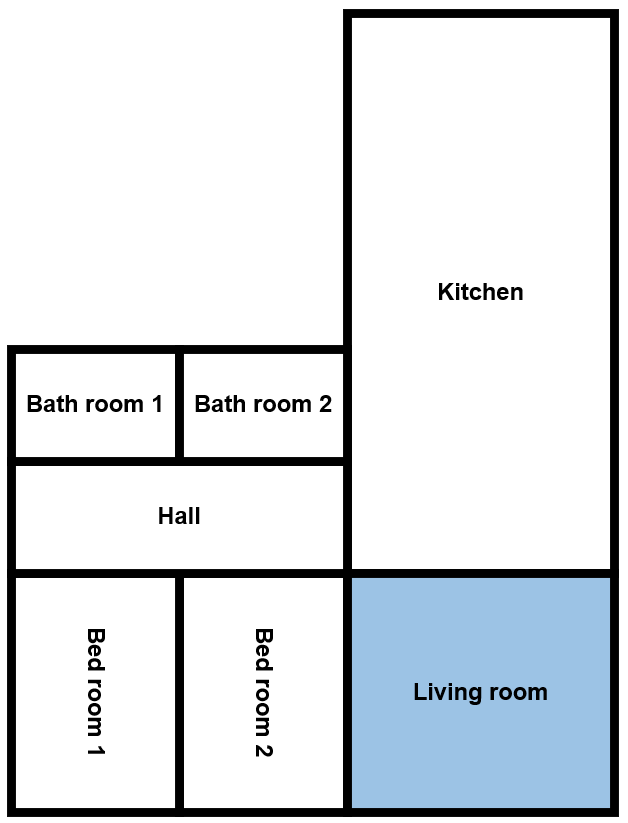
\includegraphics[width=10cm]{figures/Apartment.png}
    \caption{Network High Level Design}
    \label{fig:HLD}
\end{figure}

 The living room is 3,30m x 3,64m and aprox 12 m2. and includes furniture as shown in the figure XX. 

\begin{figure}[!ht]
    \centering
    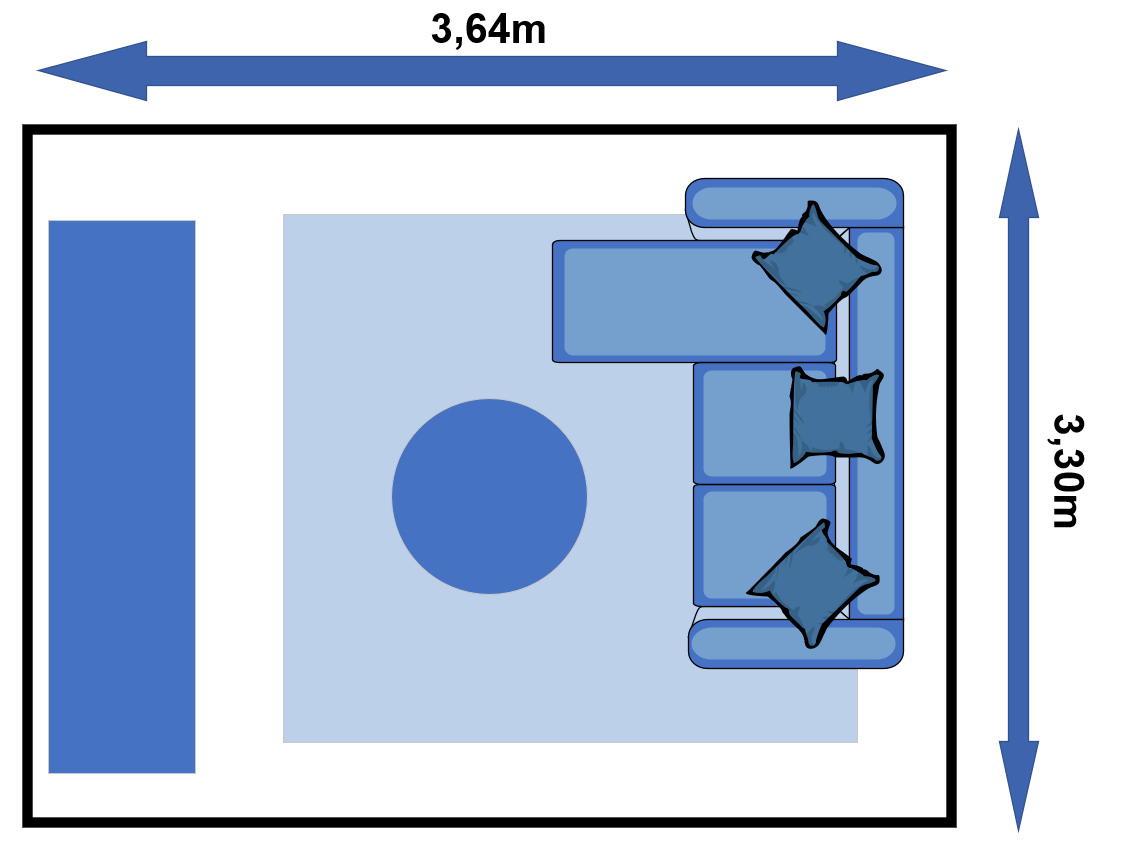
\includegraphics[width=10cm]{figures/Living room.png}
    \caption{Network High Level Design}
    \label{fig:HLD}
\end{figure}

\subsection{Robot vacuum cleaner}
The robot vacuum cleaner is the main device in this research. To select the best suited vacuum cleaner we did a selection survey which based on the requirements we had about different smart home features, price, norwegian distributor and popularity. The survey selected resulted in Irobot roomba 7i as the best option. The selection process and secifications for Irobot roomba i7 is described in subsections below.

\subsubsection{Robot vacuum selection}
Because of limited resources and time, the selection of equipment needs to be done before acquiring anything. The vacuum will need several smart home features so that the different features can be identified in the network traffic analysis. The purpose of this research is to identify how much private information which can be gathered as well as how complex these types of sniffing attack will have to be. Selecting a vacuum cleaner with more smart home features will potentially reveal more sensitive private information.

    \paragraph{Communication network protocols:} IoT devices can use several different network protocols and technology to communicate with other devices. We distinguish between Datalink layer (layer 2), Network layer (layer 3), session layer (layer 4) and Application layer (layer 5). Each of these layers can reveal different information about the session, devices and data which is sent. The Data Link Layer protocol IEEE 802.11 (Wi-Fi) it is the most widespread infrastructure in smart homes \cite{robotsel1}. Wi-fi will therefore be the preferred data link layer protocol, this to ensure the most relevant result \cite{robotsel2}\cite{robotsel3}. The selection of IEEE 802.11 will result in more common Internet routing protocols which supports the principle.

    \paragraph{App features:} To enable the best user experience possible more and more IoT devices comes with dedicated application for command, control, statistics, and integration. Such applications add new smart home features to devices which often result in more data transfers between the device and the cartelized controller. The application architecture is dependent on the vendor, but a common design is a client-server architecture, where both the vacuum cleaner and mobile application is acting as clients \cite{robotsel4}. This may include sensitive private information transferred between the devices. \cite{robotsel7}

    \paragraph{Navigation:}A robot vacuum cleaner will have to navigate around the smart home to be able to clean sufficiently. This navigation is handled differently, form the basic to more advanced navigation. Some of the more advances navigation systems uses laser or camera to navigate and map the environment. \cite{robotsel5} \cite{robotsel6} This type of mapping could generate some interesting information for the research. 

\paragraph{}Open-source information, tests sites and YouTube videos are used to gather information to base the selection on. To limit the number of relevant robot vacuum cleaner vendors I used open source review sites to determine which vendors that had the highest ranking robots. Next, I used Google Play and the available statistics to see how many downloads and rating the different vendor specific application had. Based on the results from these findings I filtered the vendor models based on app features and navigation described in the introduction, the best suited robot vacuums per vendor is then compared to each other to finally select one. Prices are gathered from the comparison website prisjakt.no\cite{prisjakt.no}. 

 From opensource test sites there was two robot vacuum vendors which did good, Irobot and Roborock, these are therefore the main vendors to be considered. As reference to another popular vendor Xiaomi is also included in the survey.\cite{robotsel11}\cite{robotsel12}\cite{robotsel13}

\paragraph{Selection:} \cite{robotsel11}\cite{robotsel12}\cite{robotsel13} is used as vendor comparison review sites, these were selected because they were some of the top results on my google with the search string “Robot vacuum cleaner test”. The vendor on top ten selection \cite{robotsel11} is listed in tabel XX, \cite{robotsel12} listed in tabel XX and \cite{robotsel13} listed in tabel XX. 

\begin{table}[]
\begin{tabular}{|l|c|}
\hline
Vendor   & Number on top ten \\ \hline
Roborock & 3                 \\ \hline
Irobot   & 3                 \\ \hline
ILife    & 2                 \\ \hline
Wyze     & 1                 \\ \hline
Neato    & 1                 \\ \hline
\end{tabular}
\end{table}


\begin{table}[]
\begin{tabular}{|c|c|}
\hline
Vendor    & Number on top ten \\ \hline
Ecovacs   & 2                 \\ \hline
Irobot    & 2                 \\ \hline
Roborock  & 2                 \\ \hline
Shark     & 1                 \\ \hline
Eufy      & 1                 \\ \hline
ILife     & 1                 \\ \hline
Proscenic & 1                 \\ \hline
\end{tabular}
\end{table}

\begin{table}[]
\begin{tabular}{|c|c|}
\hline
Vendor   & Number on top ten \\ \hline
Irobot   & 2                 \\ \hline
Roborock & 2                 \\ \hline
Neatsvor & 3                 \\ \hline
Ecovacs  & 1                 \\ \hline
Neato    & 1                 \\ \hline
Kyvol    & 1                 \\ \hline
\end{tabular}
\end{table}

\begin{table}[]
\begin{tabular}{|c|c|}
\hline
Vendor    & Number on top ten \\ \hline
Irobot    & 7                 \\ \hline
Roborock  & 7                 \\ \hline
Neatsvor  & 3                 \\ \hline
Ecovacs   & 3                 \\ \hline
ILife     & 3                 \\ \hline
Neato     & 2                 \\ \hline
Proscenic & 1                 \\ \hline
Wyze      & 1                 \\ \hline
Shark     & 1                 \\ \hline
Eufy      & 1                 \\ \hline
Kyvol     & 1                 \\ \hline
\end{tabular}
\end{table}

To get a briefly overview of the popularity of the different robot vacuum cleaners we can use the number of downloads of the different applications. This information is available in Google play with overall user rating, application rating is also available in Apples App Store. 

\begin{table}[]
\begin{tabular}{|c|c|c|}
\hline
Application & Google play download & App rating 0-5 \\ \hline
Irobot      & 5 million+           & 4,0            \\ \hline
Roborock    & 1 million +          & 4,6            \\ \hline
Xiaomi      & 10 million +         & 4,3            \\ \hline
Ecovacs     & 1 million +          & 2,5            \\ \hline
Shark       & 1 million +          & 3,3            \\ \hline
Eufy        & 1 million +          & 4,6            \\ \hline
ILife       & 10 thousand +        & 2,2            \\ \hline
Wyze        & 1 million +          & 4,0            \\ \hline
Proscentic  & 100 thousand +       & 2,0            \\ \hline
\end{tabular}
\end{table}

As we can see the most downloaded applications in google play is “Irobot” and “Xiaomi”, the difference between these two applications is that Irobot is a pure vacuum cleaner application and Xiaomi is a smart home application where you can connect other IoT devices and control your integrated smart home.  
Satisfaction based on rating is also divided between the different application, applications with the rating above 3.9 is: Irobot, Roborock, Xiamoi, Eufy and Wyze. 

\paragraph{Discussion} Based on the open-source top ten site review the results showed that Irobot and Roborock was the overall best vendors on the marked. These are therefore the most relevant vendors to compare to find the most suited vacuum cleaner to our project. This assumption is also supported when it comes to the results from Google play statistics, there we can see that both Irobot and Roborock is among the highest rated and downloaded applications. These two results make us confident that a vacuum cleaner from one of these vendors will give us a popular and well used vacuum cleaner which makes the research results more relevant. 
Xiaomi is the most downloaded application in Google play with more than 10 million downloads, in difference with the applications from iRobot and Roborock the application is designed to handle an entire smart home and not just vacuum cleaners. As Xiaomi has a lot of other IoT devices on the marked this could cause more downloads which is not directly connected to the use of their vacuum cleaners. Is was also not mentioned in any of the top ten review sites which we used and is therefore not the right fit for this research. If the purpose was to analyse an entire smart home, it could be more relevant due to the integration features in the smart home application. 
Most suitable vendor vacuum: 
Irobot Roomba I7 is the most suitable model from Irobot in this research project. This is the model which includes all the smart features included through the app without extra cost associated with extra cleaning features. Compared to the I6 model I has newer hardware and support for minimal cost. \cite{robotsel9}

\paragraph{Conclution} Both iRobot Roomba i7 and Roborock has a lot of the same features which is must have on a robot vacuum cleaner, as well as they are in the same price range. The advantage of 5 million downloads vs Roborock’s 1 million indicated that the iRobot vacuum cleaners are more used combined with smart home features. The iRobot also has seasonal and pet detection and can make suggestions on the cleaning patters, this ability to identify user behaviour could create a lot of sensitive private information about it’s roommates. iRobot Roomba i7 will therefore be the most suitable robot vacuum cleaner for this research




\subsubsection{Network design}
To represent the general smart home in common homes the research used the existing network infrastructure in the apartment and added some components to be able to better isolate the traffic from the robot vacuum cleaner. The different elements are show in figre \ref{fig:HLD}, further each device will be described. 

\begin{figure}[!ht]
    \centering
    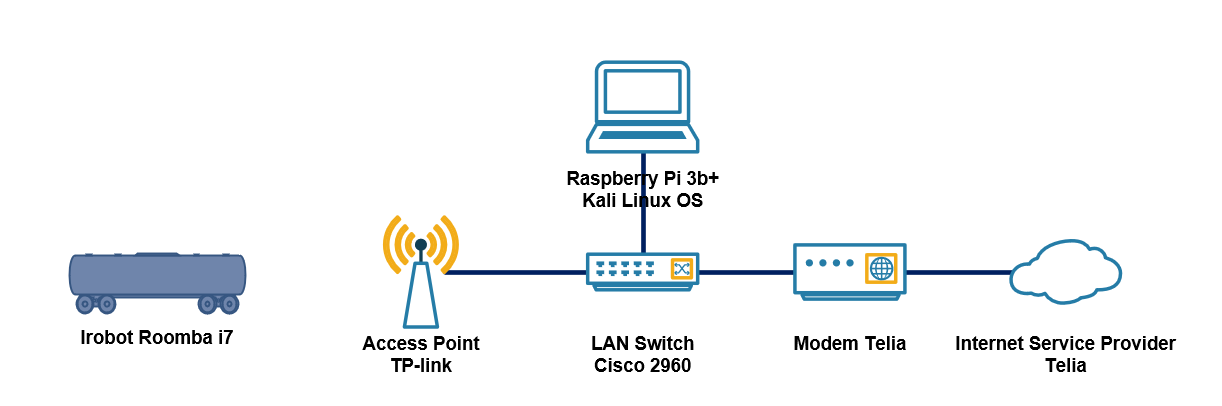
\includegraphics[width=10cm]{figures/HLD.png}
    \caption{Network High Level Design}
    \label{fig:HLD}
\end{figure}

\begin{itemize}
    \item \textbf{Device:} Raspberry Pi 3b+
    \item \textbf{Software:} Kali ARM \cite{kalidownload}, updated 27.09.2022
    \item \textbf{Configuration:}
    \begin{enumerate}
        \item Image downloaded to an external computer and written to the micro SD-card with the application balenaEtcher \cite{balenaetcherdownload}.
        \item Patching done 19.12.2022 with the command "sudo apt update \&\& sudo apt upgrade"
    \end{enumerate}
    \item \textbf{Connected items:}
    \begin{enumerate}
        \item Micro SD card \cite{microsdcard}
        \item TL-WN722N USB WiFi Adapter \cite{tp-link}
    \end{enumerate}
\end{itemize}

\section{Test cases}
Each test Case consists of a detailed test description, which enables the tests and results to be reproduced as identical as possible. It will also state how many times the test was done during the research. The standby traffic test is performed over 14 consecutive days, and all other tests are done 20 times. The number of days and tests are decided based on the available time frame for this master thesis. Equipment selection process, design and configuration process and test phase is time consuming and 20 is therefore chosen as the overall test number. 

\subsection{Baseline-traffic}
Baseline test have the function to represent the traffic flow generated by the robot vacuum cleaner installed in the smart home environment with out any event triggering. For this test the robot vacuum cleaner is installed in the chosen smart home environment described in "smart home environment chapter". Before the test was conducted the robot was operational for more then 60 days, and more then 10 cleaning jobs done. This to ensure that is is in operational mode.

\begin{itemize}
    \item \textbf{Description:} Conduct packet sniffing for both wireless and cabled traffic generated over a number consecutive days. Capture data is stored in two separate files. The Robot vacuum cleaner is connected to power and Internet the entire time period.
    \item \textbf{Number of tests:} 14 consecutive days
\end{itemize}

\subsection{Triggered cleaning}
Triggered cleaning is an event started trough the IRobot application with the use of "start cleaning". The test is done when the mobile application receives a notification that the cleaning is done. If the robot vacuum need to return to base to recharge, empty bin or get stuck something in the brushes, actions will be done to enable the robot to continue cleaning. 
\begin{itemize}
    \item \textbf{Description:} Start cleaning through the Irobot application, with the use of start cleaning. Capture is started 10 minutes before cleaning is scheduled and stopped 30 minutes after the cleaning is finished. 
    \item \textbf{Number of tests:} 20
\end{itemize}

\subsection{Empty bin} The bin needs to be removed from the vacuum cleaner to be emptied. This will make the vacuum cleaner in a state where is cannot start cleaning, and the application will display information about the situation. 

\begin{itemize}
    \item \textbf{Description:}Start packet capturing 5 minutes before the bin is removed. Remove the bin, wait 5 minutes and then insert the bin once more. Stop capturing 5 minutes after the bin is inserted
    \item \textbf{Number of tests:}20
\end{itemize}

\subsection{Open mobile application}
Mobile application will be able to access information about the robot vacuum cleaner. This might generate pull requests from the Irobot cloud towards the vacuum cleaner to get the needed information to display. If the user changes attribute in the application this needs to be communicated with the vacuum cleaner. 
\begin{itemize}
    \item \textbf{Description:} Start packet capturing 5 minutes before opening the application on the smart phone. Open the application, change a "room name" and one "room separation line", then wait until the application have been open for 5 minutes, then close the application. Stop packet capturing after additionally 5 minutes. 
    \item \textbf{Number of tests:}20
\end{itemize}



\section{Methods in relates work}
Through some one the papers review in the related work section they used to capture live traffic from the smart devices.In this section the different methods in \cite{lindaeavesdropping} \cite{eavsIoT} \cite{Neato}, will be discussed and elements that could be used in this research will be identified and justified. 


\begin{itemize}
    \item \textbf{Description:}
    \item \textbf{Number of tests:}20
\end{itemize}
\chapter*{Method - Redo}

In this chapter the method used to conduct this Master thesis will be described. The entire method is broken down into several different processes and sub processes to better structure and describe, this is illustrated in \ref{fig:Method_process}. Each individual process has an outcome which is needed as input in the next process. 

\begin{figure}[H]
    \centering
    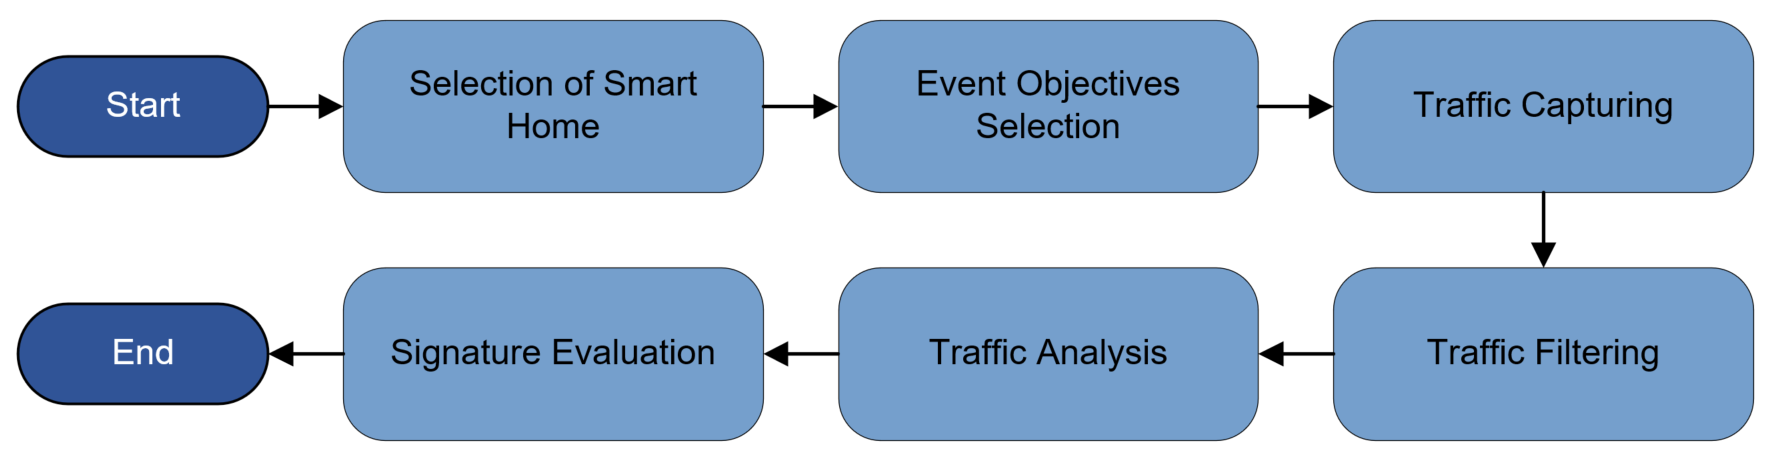
\includegraphics[width=\textwidth]{figures/Method_process.png}
    \caption{Overall phases }
    \label{fig:Method_process}
\end{figure}


\section{Device and Environment Selection}
With limited resources it is important to find the best satiable deceives for the thesis project. Since all the testing and analysis is based on the data generated by the robot vacuum cleaner, it will be selected first. To ensure that the thesis is relevant there is some requirements that is created.

\begin{figure}[H]
    \centering
    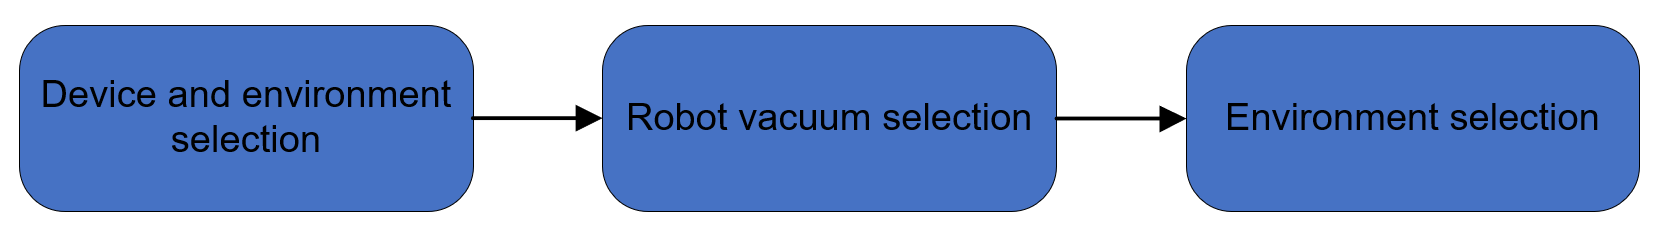
\includegraphics[width=\textwidth]{figures/DeviceSelectionProcess.png}
    \caption{Device Selection Process}
    \label{fig:DeviceSelectionProcess}
\end{figure}

\subsection{Selection Robot vacuum cleaner}
\begin{itemize}
    \item \textbf{Communication protocol:} Wi-Fi is the most wide spread communication protocol in today's IT infrastructure, as well as in Smart home \cite{robotsel1}. Eavesdropping devices and analysis tools are also more available for IEEE.802.11 and network layers higher in the OSI model \cite{osimodel}.
    
    \item \textbf{Smart Home Features:} The robot vacuum cleaner need to have several different smart home features. As more features available the more attribution and potential information can be extracted.This includes as application, which is more likely to produce traffic towards an external services, potentially exposing data \cite{robotsel4}.
    
    \item \textbf{Popularity:} The prevalence of different vendors and models will vary, and the popularity of the selected vacuum cleaner will impact the relevance of this research, the more devices used, the more smart home will be effected of the research's result. 
\end{itemize}

Data and ratings from these three robot vacuum cleaner review sites was used \cite{robotsel11}\cite{robotsel12}\cite{robotsel13}. The summary of all these reviews will be used to determine most reliable vacuum cleaner vendors. To determine the popularity of the different brands, statistics about number of downloads and ratings is gathered from Google Play \cite{GooglePlay} and compared.
Models within the assortment of the two highest scoring vendors will be compared and selected, based on the overall criteria and with the use of \cite{robotsel9}

\subsection{Result selection robot vacuum cleaner}

Results from thhe review sites shows that the two best robot vaccum cleaner vendors is Irobot and Roborock \ref{tab:RobotVacuumselcetionReviewSites}. 

\begin{table}[H]
    \centering
    \begin{subtable}[b]{0.45\linewidth}
        \centering
        \caption{Results from review-site \cite{robotsel11}}
        \label{tab:RobotReviw1}
        \begin{tabular}{|l|l|}
            \hline 
            \textbf{Vendor} & \textbf{Number on top ten} \\ \hline
            Irobot      & 3                 \\                   \hline
            Roborock    & 3                 \\                   \hline
            Neatsvor    & 0                 \\                   \hline
            Ecovacs     & 0                 \\                   \hline
            iLife       & 2                 \\                   \hline
        \end{tabular}
    \end{subtable}
    \hspace{0.5cm}
    \begin{subtable}[b]{0.45\linewidth}
        \centering
        \caption{Results from review-site \cite{robotsel12}}
        \label{tab:RobotReviw2}
        \begin{tabular}{|l|l|}
            \hline
            \textbf{Vendor}    & \textbf{Number on top ten} \\ \hline
            Irobot      & 2                 \\                   \hline
            Roborock    & 2                 \\                   \hline
            Neatsvor    & 0                 \\                   \hline
            Ecovacs     & 2                 \\                   \hline
            iLife       & 1                 \\                   \hline
        \end{tabular}
    \end{subtable}
    \begin{subtable}[b]{0.45\linewidth}
        \centering
        \caption{Results from review-site \cite{robotsel13}}
        \label{tab:RobotReviw2}
        \begin{tabular}{|l|l|}
            \hline
            \textbf{Vendor}    & \textbf{Number on top ten} \\ \hline
            Irobot      & 2                 \\                   \hline
            Roborock    & 2                 \\                   \hline
            Neatsvor    & 3                 \\                   \hline
            Ecovacs     & 1                 \\                   \hline
            iLife       & 0                 \\                   \hline
        \end{tabular}
    \end{subtable}
    \hspace{0.5cm}
    \begin{subtable}[b]{0.45\linewidth}
        \centering
        \caption{Summary of all review-sites}
        \label{tab:RobotReviw2}
        \begin{tabular}{|l|l|}
            \hline
            \textbf{Vendor}    & \textbf{Number on top ten} \\ \hline
            Irobot      & 7                 \\                   \hline
            Roborock    & 7                 \\                   \hline
            Neatsvor    & 3                 \\                   \hline
            Ecovacs     & 3                 \\                   \hline
            iLife       & 3                 \\                   \hline
        \end{tabular}
    \end{subtable}
    \label{tab:RobotVacuumselcetionReviewSites}
    \caption{Robot vacuum selection review-site}
\end{table}

Application related different vendors' robot vacuum cleaner is presented in \ref{tab:VendorApplicationStat}. It is worth mentioning that the "Smart Life" application used to control the Neatsvor is used to integrate the entire smart home and not just a robot vacuum cleaner. 

\begin{table}[H]
\centering
\caption{Vendor application statistics}
\label{tab:VendorApplicationStat}
\begin{tabular}{|c|c|c|c|}
\hline
\textbf{Vendor} & \textbf{Application} & \textbf{Downloads} & \textbf{Rating} \\ \hline
Irobot          & Irobot Home          & 5 million +        & 4,0/5,0         \\ \hline
Roborock        & Roborock             & 1 million +        & 4,6/5,0         \\ \hline
Neatsvor        & Smart Life           & 10 million +       & 4,5/5,0         \\ \hline
Ecovacs         & Ecovacs Home         & 1 million +        & 2,5/5,0         \\ \hline
iLife           & iLifehome            & 50 thousand +      & NA              \\ \hline
\end{tabular}
\end{table}
Both Irobot and Roborock received seven recommendations, which was significantly higher than the other three vendors on the list, each of which had only three representations. Additionally, both vendors were referenced in all three review sites, which strengthens their credibility. 

In the application download and ratings analysis, the Neatsvor application had over 10 million downloads. However, this application is more focused on smart home integration, and the high number of downloads is likely not solely due to the robot vacuum cleaner. Meanwhile, Evacos home received a 2.5/5.0 rating, and despite having a similar number of downloads as Roborock, it fell short in the selection process. Hence, Irobot and Roborock emerged as the two most relevant vendors. In a comparison of their products, it was found that the Irobot Roomba i7 and Roborock S6 were the best suitable robots according to our requirements \cite{robotsel8} \cite{robotsel6}. The comparison was conducted using the website \cite{robotsel9}, which is presented in Table \ref{tab:IrobotRoborockComparison}.

\begin{table}[H]
\centering
\caption{Irobot and Roborock comaprison}
\label{tab:IrobotRoborockComparison}
\begin{tabular}{|p{0.45\textwidth}|p{0.45\textwidth}|}
\hline
\multicolumn{1}{|c|}{\textbf{Irobot roomba i7}}        & \multicolumn{1}{c|}{\textbf{Roborock s6}}                \\ \hline
Camera   and odometry for navigation                   & Map   discovery, and storage of floorplan                \\ \hline
Cleaning   suggestions by the application              & Scheduling                                               \\ \hline
Zone   based cleaning                                  & No   map zones, mapping zones                            \\ \hline
Seasonal   cleaning                                    & Real-time   tracking                                     \\ \hline
Pet   detection                                        & LDS   sensor for mapping and navigation                  \\ \hline
SRR   rating App features 71, Usability and control 69 & SRR   rating: App features 100, Control and usability 71 \\ \hline
Price:   3990kr                                        & Price:   3990kr                                          \\ \hline
\end{tabular}
\end{table}

Irobot roomba i7 and Roborck S6 have similar reviews and rating all over, and they both have a sufficient number of smart home features required in this thesis. The fact that the Irobot application is downloaded 5 times more than the Roborock was the decisive factor, and Irobot roomba i7 will be used during this research. 

\subsection{Environment selection}
The rest of the research environment have to support and allow traffic eavesdropping and analysis, of the Irobot Roomba i7.  Important factors to support in research environment:

\begin{itemize}
    \item \textbf{IEEE.802.11 WI-FI network}
    \item \textbf{Internet connection}
    \item \textbf{Different physical rooms}
\end{itemize}

\subsubsection{Physical environment}
To ensure the validity of the results across diverse settings, the testing will be conducted in two different home environments situated in separate cities. The Robot vacuum cleaner will be configured from factory defaults for each research environment. Both home environments have independent Internet access, provided by distinct external Internet Service Providers (ISPs). To control the duration of each test, the trials will be restricted to the room with the ISP router. As the floor space in this room is smaller, the cleaning process will be relatively shorter. An illustration of the two distinct smart home environments is provided below in \ref{fig:SmartHomeEnvironments}.

\begin{figure}[H]
    \centering
    \begin{subfigure}[b]{0.80\textwidth}
        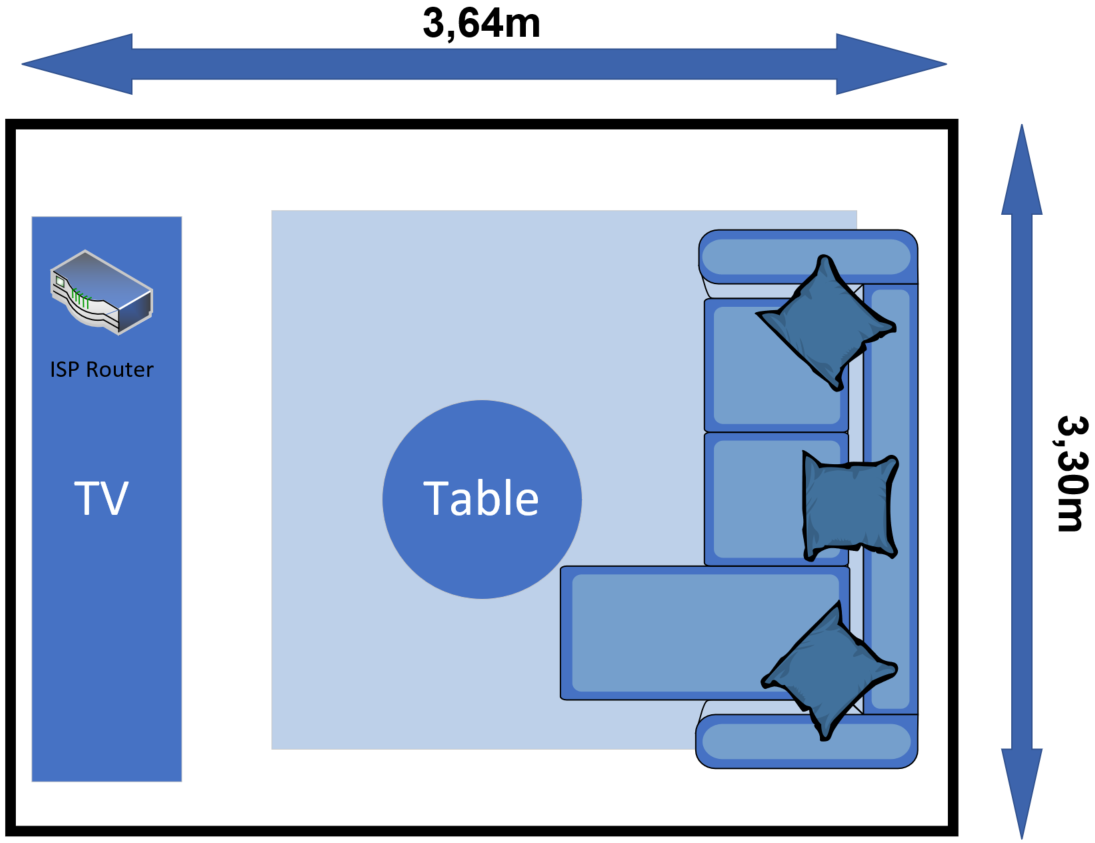
\includegraphics[width=\textwidth]{figures/Environment1.png}
        \caption{Research environment 1}
        \label{fig:Environment1}
    \end{subfigure}
    \hfill
    \begin{subfigure}[b]{0.80\textwidth}
        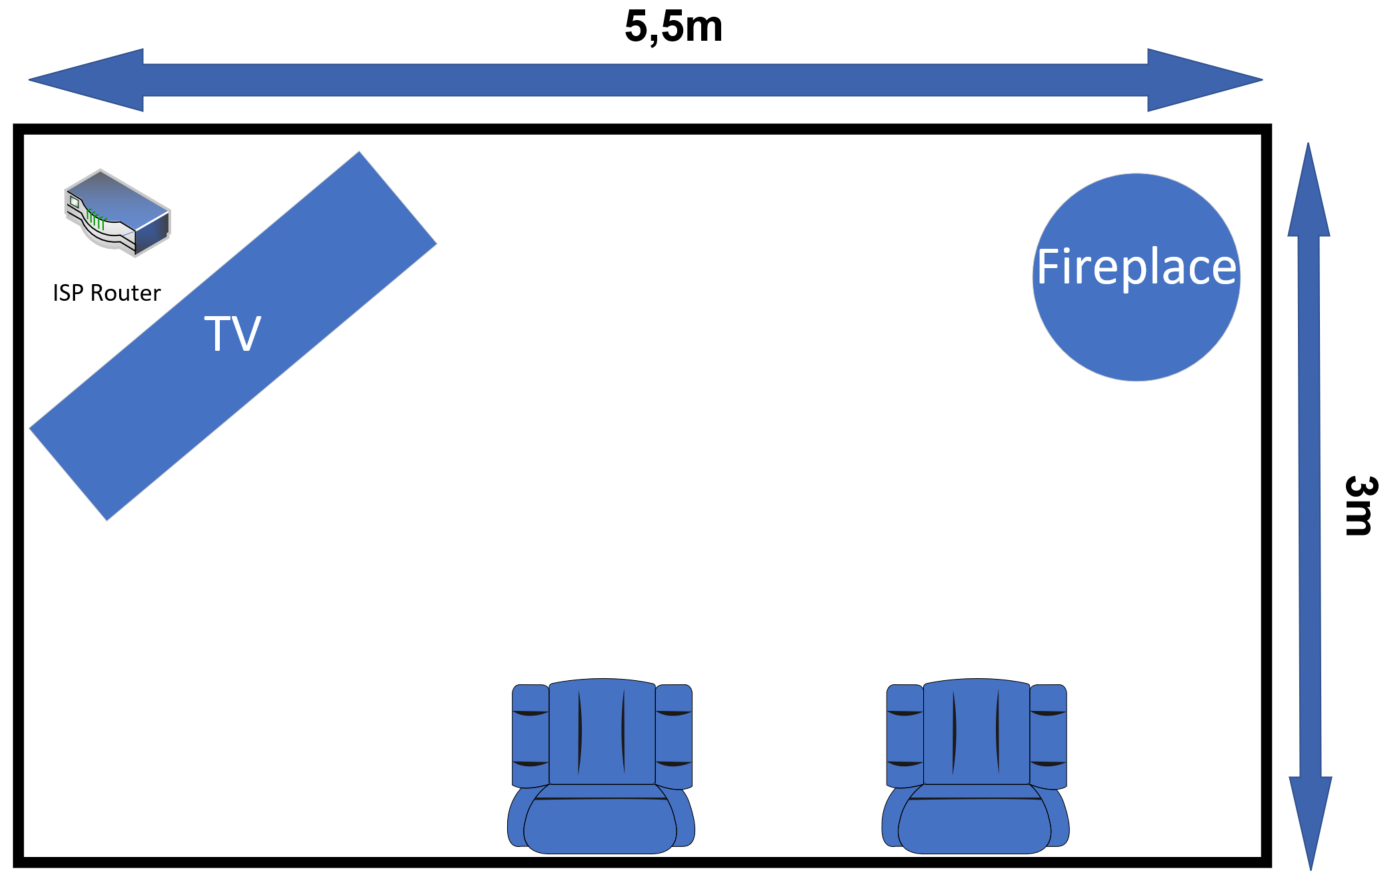
\includegraphics[width=\textwidth]{figures/Environment2.png}
        \caption{Environment 2}
        \label{fig:Environmet2}
    \end{subfigure}
    \caption{Smart Home environments }
    \label{fig:SmartHomeEnvironments}
\end{figure}

\subsubsection{Capturing and Analysis platform}
For the capturing and analysis platfrom there is some requirements that needs to be fulfilled. Due to limited resources the platforms need to be available for limited cost. 

\begin{itemize}
    \item \textbf{Capturing platform} needs to be able to operate autonomously, due to continuously capturing of events. It needs software that enables capturing of wireless IEEE.802.11 and wired traffic IEEE.802.3 at the same time. This data will need to be transferred from the device to the analysis platform.
    \item \textbf{Analysis platform} needs to have tools analysis the traffic, based on the format of the capturing tool. 
\end{itemize}

As capturing platform the Raspberry PI 3b+ is chosen, this was available form free through the authors' employer. This device is created to run autonomous, as OS the Kali Linux is installed. This is a open source operating system, including several different tools to capture and analyse traffic and has has an OS-version designed for Raspberry PI \cite{kalidownload}. To enable capturing of wireless traffic the wireless network interface card needs to be in \textit{Monitor mode}. For Kali Linux the \textit{LINK TL-WN722N V2/V3} is recommended by \cite{Kali_monitormode_guide}, and is therefore used in this research. 
Analysis platform is a HP Elitebook due to availability. Is runs Windows 11 OS which is compatible with several different tools for capturing and analysis.

\subsubsection{Environment infrastructure}
This research will include eavesdropping of wireless traffic and wired WAN traffic. The two different smart home environments only includes a single ISP router providing both Internet connection and Wi-Fi, and does not have a features allowing the captuing platfrom to eavsdropp the wired traffic generated by the robot vacuum cleaner. Additional infrastructure is therefore added: 
\begin{itemize}
    \item \textbf{Wireless access point:} This access point will create a new SSID only to be used by the Robot vacuum cleaner, this isolates the vacuum cleaner from potential impact from other devices on the WLAN/LAN. The access point will also use Network address translation and translate all traffic to one singe IP address. With this setup, all traffic with the source address of the access point will be either the access point itself, or the robot vacuum cleaner.
    \item \textbf{LAN switch:} The LAN switch will be directly connected to both the access point and the ISP router. All Internet traffic will therefore be transmitted though the switch. A SPAN port is configured on the switch, this port will monitor all traffic on the port connected to the access point, and duplicate this flow to the port connected to the capturing platform. This setup is illustrated in \ref{fig:WLAN_LAN_setup}
\end{itemize}

\begin{figure}[H]
    \centering
    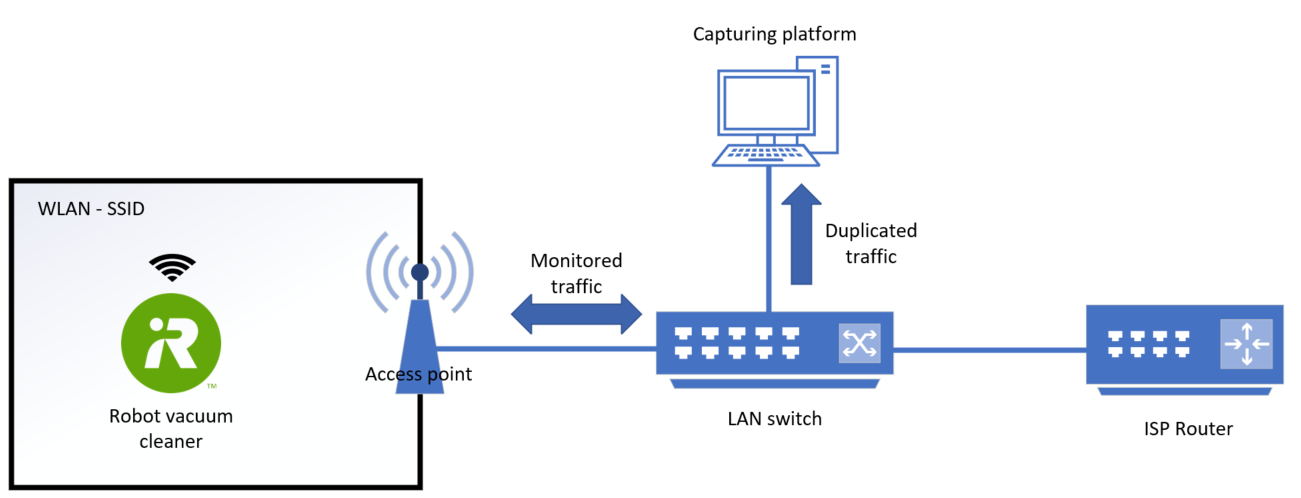
\includegraphics[width=\textwidth]{figures/WLAN_LAN_setup.png}
    \caption{Smart Home infrastructure}
    \label{fig:WLAN_LAN_setup}
\end{figure}



\subsubsection{Capturing and Analysis tools}
Capturing and analysis tools need to be compatible with each other. Stored format from the capturing process needs to be readable in the analysis phase. Tools for these kinds of tasks are many. Whireshark is a widely used network protocol analyser, it allows network capturing and analysis in real-time. It can be used for deep header inspection in all network layers which is not encrypted before the capturing, this makes it a valuable tool for network and security purposes. The application can perform basic identification of a wide range of different protocols across networks layers as well as statistics about the traffic flow. This software is also default installed on Kali Linux OS. Wireshark is also available for Windows on \cite{wireshark_download_2016}.
Tshark is a sub-software included in wireshark and the process which is used to capture traffic on the dedicated network interfaces. This software can be used to capture traffic through CLI. In this process it is possible to define capturing filters which only store traffic that is interesting for the analysis phase.


\section{Traffic capturing}
This section will describe the tools used for traffic capturing, tests and the process of how the capturing process is executed. All capturing will be executed on the capturing platform, both LAN and WLAN traffic is captured simultaneously. This enables correlation of the traffic for the same event.  

\begin{figure}[H]
    \centering
    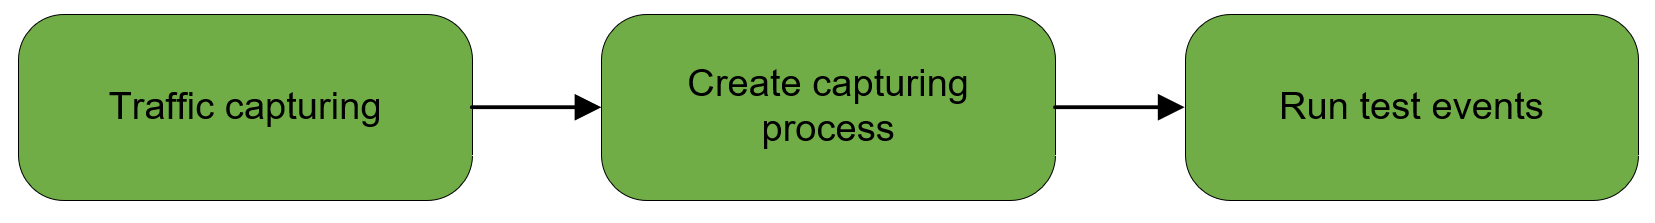
\includegraphics[width=\textwidth]{figures/TrafficCapturingProcess.png}
    \caption{Traffic Capturing Process}
    \label{fig:TrafficCapturingProcess}
\end{figure}

\subsection{Captuing tools}
Tshark will be used as the capturing tools for both wireless and wired traffic. Two Tshark instances will run simultaneously on the capturing platform. The Tshark filter syntax used for both capturing streams is: 
\\
tshark [ -i <capture interface>|- ] [ -f <capture filter> ] [ -w <outfile>|- ]
\\
The captuing platform has three different NICs:
\begin{itemize}
    \item \textbf{eth0,} is the wired IEEE 802.3 interface which is connected to the SPAN port of the LAN switch.
    \item \textbf{wlan0,} is the buildt in IEEE 802.11 interface on the Raspberry PI.
    \item  \textbf{wlan1,} external IEE 802.11 adapter which is configured to monitor mode.
\end{itemize}

LAN Tshark command:
\\
sudo tshark -i wlan1 -f 'ip.host "WAN address' -w output.pcap
\\
WLAN Tshark command:
\\
sudo tshark -i wlan1 -f 'eth.host "MAC address' -w output.pcap
\\

\subsection{Capturing process}
The capturing process will be similar for all events, this will create a better foundation to compare the different test results. \ref{fig:captuingprocess} illustrate the entire process.
\begin{enumerate}
    \item Star both LAN and WLAN capture, in separate Tshark processes.
    \item Trigger events according to test event matrix. Note event Start and End during the testing. 
    \item If pcap file exceeds 500MB, stop capture, and start new LAN and WLAN capture.
    \item When testing in environment is finished, stop capture. 
    \item Transfer files to analysis platform
\end{enumerate}
   

\begin{figure}[H]
    \centering
    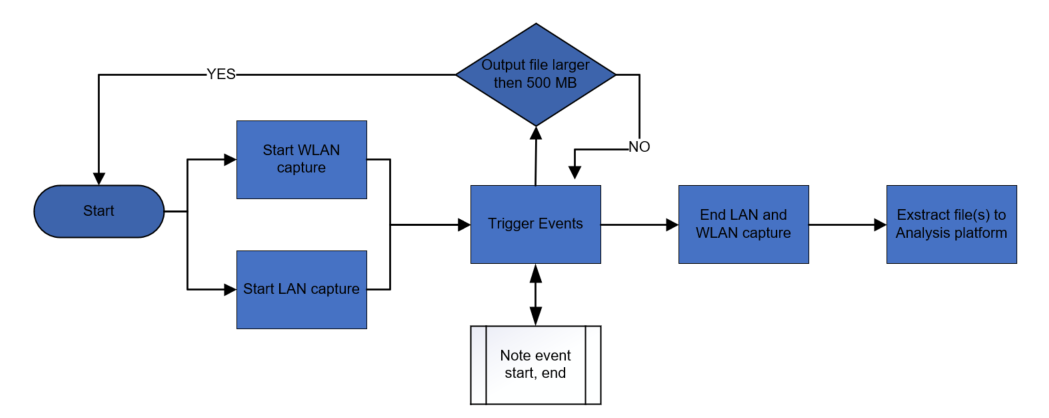
\includegraphics[width=\textwidth]{figures/Event triggering process.png}
    \caption{Capturing process}
    \label{fig:captuingprocess}
\end{figure}

\subsection{Events tests}
This section will describe the different features that is included in the research and the overall event triggering process. Each test will be executed at least n times for each of the two environments. N is the number of event which is decided to be sufficient to extract signatures with human manual analysis. The overall event triggering process is illustrated in \ref{fig:EventTriggeringProcess}

\begin{figure}[H]
    \centering
    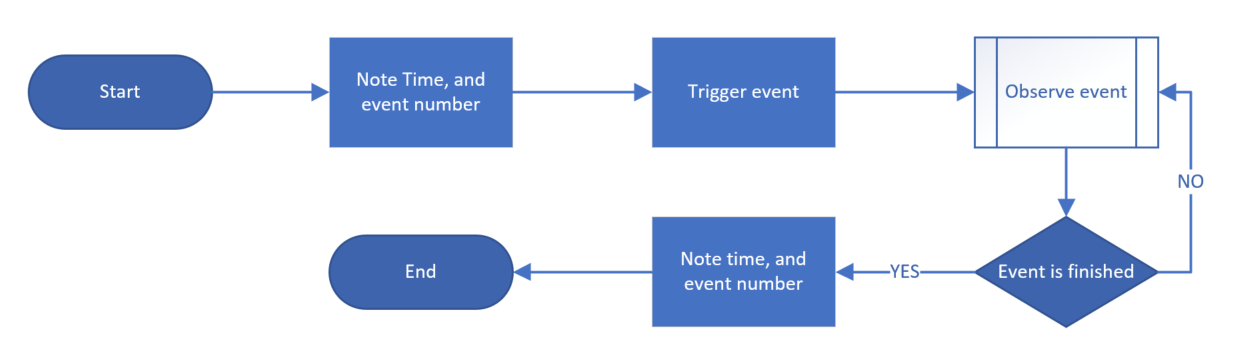
\includegraphics[width=\textwidth]{figures/EventTriggeringProcess.png}
    \caption{Capturing process}
    \label{fig:EventTriggeringProcess}
\end{figure}

\subsection{Event tests}
In this section all the different test flows will be described. This will make the tests and results more reproducible. 

\subsubsection{Standby Traffic}
This test is executed to identify network traffic generated to the robot vacuum cleaner in a standby mode. This means that there is no interaction done by human. 

\begin{itemize}
    \item \textbf{Event flow} \begin{enumerate}
                                    \item Start captuing of LAN and WLAN traffic
                                    \item Wait 14 days without any human interaction
                                    \item Stop capturing
                                \end{enumerate}
    \item \textbf{Number of events:} 1
\end{itemize}

\subsubsection{Scheduled Cleaning}
Scheduled cleaning can be configured through the application. Users can schedule a cleaning, specifying area in the smart home, time which the cleaning should start, as well as how often this should occur. 
\begin{itemize}
    \item \textbf{Event flow} \begin{enumerate}
                                    \item Schedule cleaning outside of event capture
                                    \item Note the time when cleaning started
                                    \item Note when "finished cleaning" notification is received
                                \end{enumerate}
    \item \textbf{Number of events in each environment:} 10
\end{itemize}

\subsubsection{Automated cleaning}
Irobot has features to integrate other services as triggers for events. This includes IFFF location tracker, Agust smart lock system, ecobee termotat system, My Leviton smart home integration and MyQ garage system. In this research the IFFF location system will be used. Cleaning is then triggered when the users phone is x meters away from home, where x is between 100m and 1 km. 

\begin{itemize}
    \item \textbf{Event flow} \begin{enumerate}
                                    \item Configure automated cleaning outside of event capture
                                    \item Leave the smart home environment
                                    \item Note when cleaning notification is received
                                    \item Note when "finished cleaning" notification is received
                                \end{enumerate}
    \item \textbf{Number of events in each environment:} 10
\end{itemize}

\subsubsection{Application triggered cleaning}
In the application users can trigger cleaning. There is a predefined "clean all" option, if the user have not customized. Cleaning is triggered when the user is pressing a cleaning option in the application.

\begin{itemize}
    \item \textbf{Event flow} \begin{enumerate}
                                    \item Note time
                                    \item Open the application and trigger "clean all" event
                                    \item Note when "finished cleaning" notification is received
                                \end{enumerate}
    \item \textbf{Number of events in each environment:} 10
\end{itemize}

\subsubsection{Physical triggered cleaning}
The Irobot roomba i7 has a physical cleaning button on top of the vacuum cleaner. A "clean all" vent is triggered when this button is pressed.

\begin{itemize}
    \item \textbf{Event flow} \begin{enumerate}
                                    \item Note time
                                    \item Press the physical clean button on the vacuum cleaner
                                    \item Note when "finished cleaning" notification is received
                                \end{enumerate}
    \item \textbf{Number of events in each environment:} 10
\end{itemize}

\subsubsection{Open application}
When the application is opened information will be displayed, through the application the user can interact and change setting. 

\begin{itemize}
    \item \textbf{Event flow} \begin{enumerate}
                                    \item Note time
                                    \item Open the application on the smart phone
                                    \item wait for some time
                                    \item Close application
                                    \item Note time
                                \end{enumerate}
    \item \textbf{Number of events in each environment:} 10
\end{itemize}

\subsubsection{Remove bin}
The Irobot roomba i7 has it own bin where dust is collected during clean. This can be removed if it is to be empty. The user will then have to physically remove and insert again. 

\begin{itemize}
    \item \textbf{Event flow} \begin{enumerate}
                                    \item Note time
                                    \item Remove the bin
                                    \item wait ta least 40 seconds
                                    \item Insert the bin
                                    \item Note time
                                \end{enumerate}
    \item \textbf{Number of events in each environment:} 10
\end{itemize}

\section{Traffic processing}
To make the processing feasible for the human mind there will be conducted some pre processing and filtering of the data. The standby traffic capture will be used for the initial processing, all traffic in this capture is either generated by the Access point or the robot vacuum cleaner. This initial processing will be done in Wireshark. Reoccurring traffic in the Standby capture can be filter out since they are not directly connected to an event that is triggered. All the identified traffic flows not relevant to events will be added to Wireshark capture filter \cite{wireshark}, and excluded from the display.

\begin{figure}[H]
    \centering
    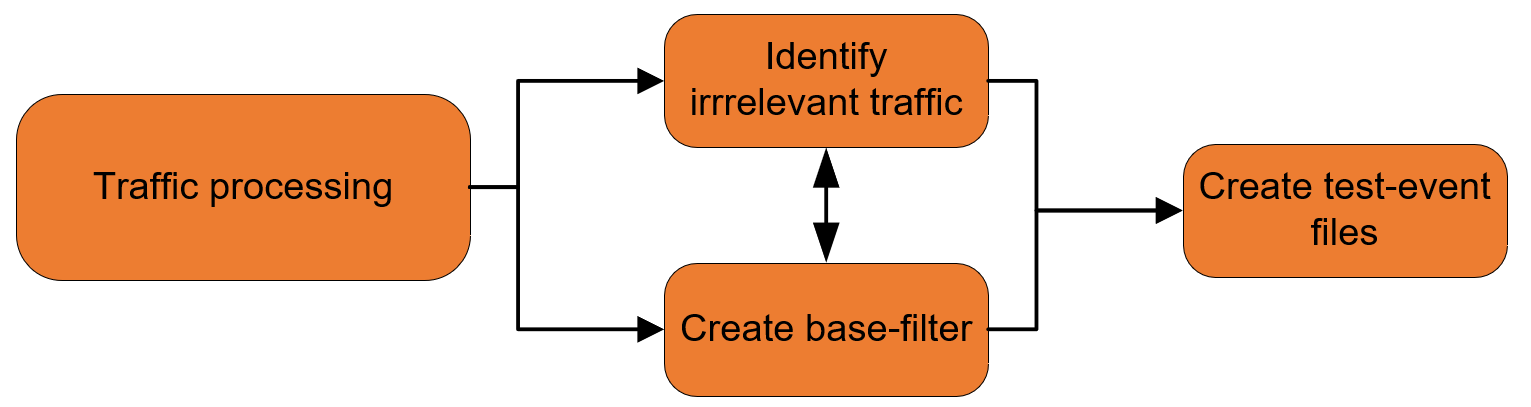
\includegraphics[width=\textwidth]{figures/TrafficProcessingProcess.png}
    \caption{Traffic processing Process}
    \label{fig:TrafficProcessingProcess}
\end{figure}


The Wireshark filter will be created with a series of if statements combined in a logical AND, or , not system. Each irrelevant traffic flow will be added to this combined filter. At the end of pre-processing a time filter will be added to create individual pcap files per event. This is to isolate the events in the analysis phase, this filter will use event start and end which was stored in the traffic capturing process. 

\textit{(frame.len >= " Month day, start-time") \&\& (frame.len <= "Month day, end-time")}

\begin{figure}[H]
    \centering
    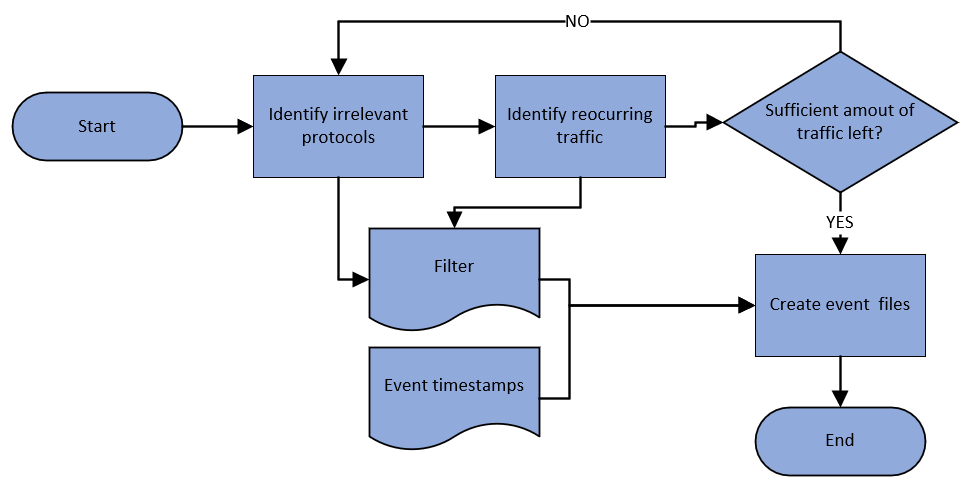
\includegraphics[width=\textwidth]{figures/TrafficprocessingFilter.png}
    \caption{Capturing process}
    \label{fig:<trafficProcessFilter}
\end{figure}

\section{Traffic Analysis}
The traffic analysis will be divided into three different processes, \textit{protocol and event relation, Traffic sequence identification and Overall event characteristics}. 

\begin{figure}[H]
    \centering
    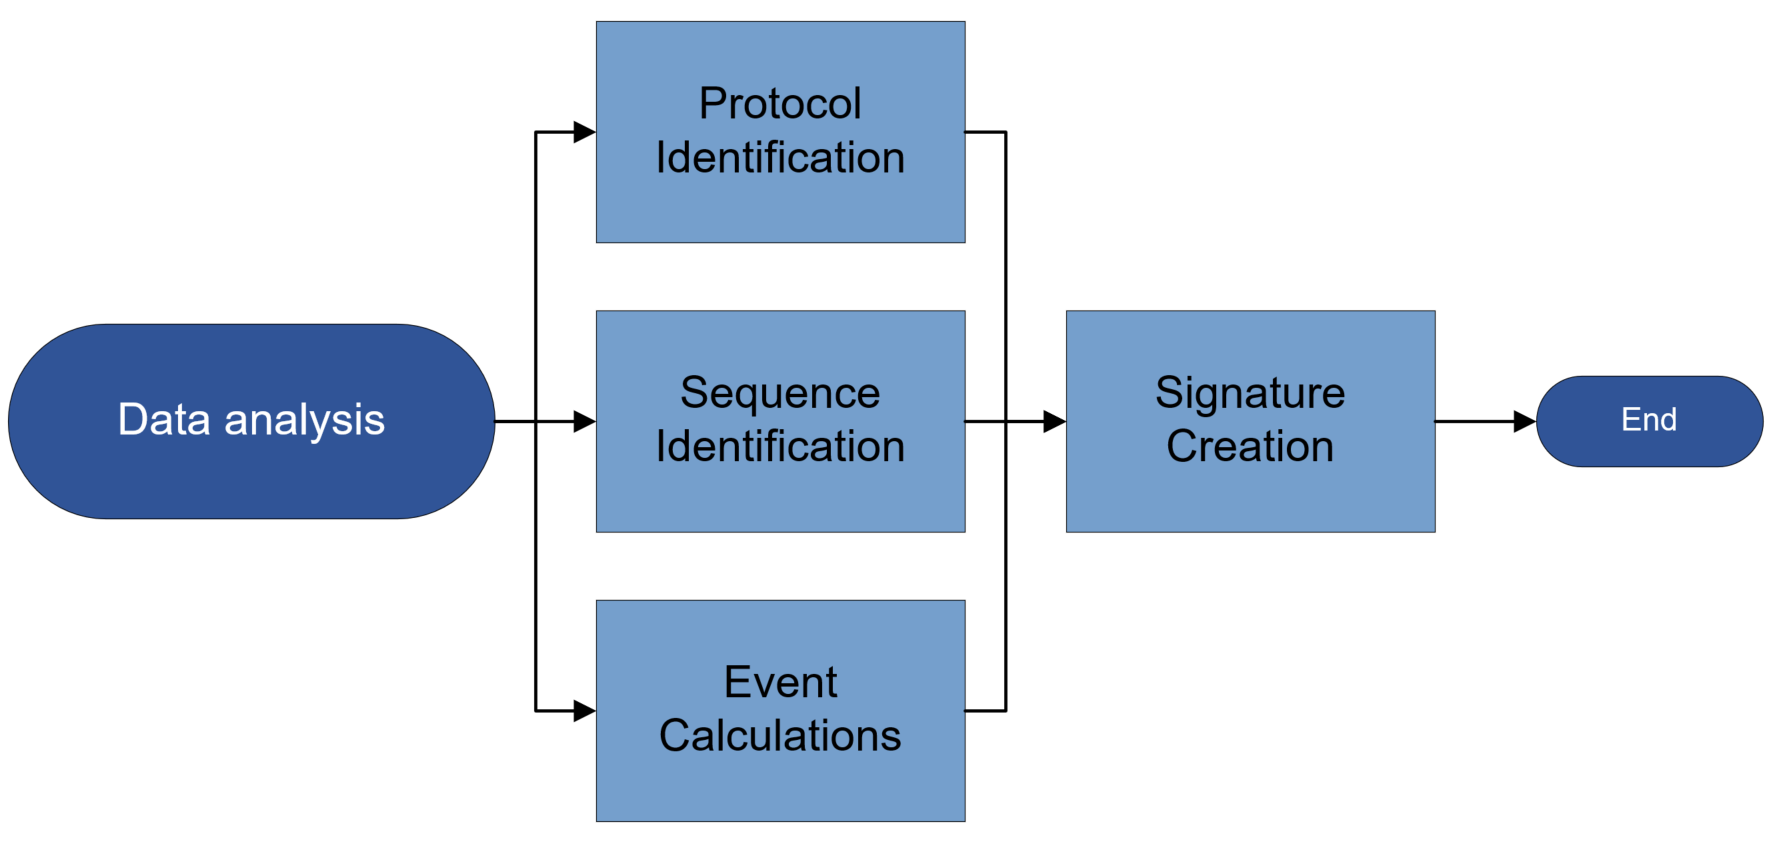
\includegraphics[width=\textwidth]{figures/TrafficAnalysisProcess.png}
    \caption{Traffic Analysis Process}
    \label{fig:TrafficAnalysisProcess}
\end{figure}

\subsection{Protocol event relation}
In this process Wireshark will be used to identify the different protocols in each event. Each identified protocol will then be looked at individually first, before combining findings in the overall event.

\subsection{Traffic sequence}
Other researches have used attributes in captured traffic flow to identify events. In this process the same approach as used in \cite{pingpong} will be done. Packet lengths around the time where the event was triggered. Three different types will be extracted: 
\begin{itemize}
    \item Packet lengths both directions.
    \item Packet lengths with Vacuum cleaner as source.
    \item Packet lengths with vacuum cleaner as destination.
\end{itemize}

\subsection{Overall event characteristics}
Each event has an overall characteristics, this data will be extracted and compared against the other event files. The data which will be compared is: 
\begin{itemize}
    \item Number of packets
    \item Total bytes
    \item Total bytes sent from vacuum cleaner
    \item Total bytes received as vacuum cleaner
    \item Different protocols
\end{itemize}

\subsection{Event signatures}
The output from the different identification processes will be compared and used to create suggestion for event signatures. These signatures will be created as conditions in a python script, and applied to the different event files to see if it is possible to identify the same signature in the event file. 
If the event is identified, the signature is testet on the other evetns' files to see if it will generate false positive. If the signature results in a success rate higher then x, it will be consider to be possible to identify. The logic will follow sudo code:
\\ 
\begin{lstlisting}
# Python code, Signeture detection
1. def Identify_event(event_file, event_confidence_variable):
2.     event_siganture = ['siganture']
3.     if event_signature is in eventfile:
4.         event_confident_variabel =+ x
5.     else
6.         None
7.     return evenr_confodence_variabel
\end{lstlisting}

\section{Signature detection and evaluation}
All signatures with higher success rate then x, will be included in the Human-learn:rule-based script. The detection algorithm has limitations, and can only identify one event per pcap file. For each event there will be a function checking for an event signature in the imported pcap file. It will follow this logic:
\\

\begin{lstlisting}
# Python code, Signeture detection
1. Main()
2.      #import event pcap file
3.      Capture = import(Event_file_x)
4.      #Run detection functions, and create confidence variables
5.      #eventX_confident_variable = eX_cv  
6.      e1_cv = identify_event1(Capture, event1_confodence_variable)
7.      e2_cv = identify_event2(Capture, event1_confodence_variable)
8.      e3_cv = identify_event3(Capture, event1_confodence_variable)
9.      e4_cv = identify_event4(Capture, event1_confodence_variable)
10.     e5_cv = identify_event5(Capture, event1_confodence_variable)
11.     e6_cv = identify_event6(Capture, event1_confodence_variable)
12.     #comapre event_confident_variables highest is event
13.     confident_variables = [list of all variables]
14.     for event in range(1,6)
15.          if confidentvariabels[event] is larger then last number
16.              largest = confidentvariabels[event]  
\end{lstlisting}

\subsection{Evaluation}
After completing the analysis and creating signature detection rules, a evaluation test will be done. The robot vacuum cleaner will be run in three new environment with, form factory defaults. Each event will be executed one time per new evaluation environment, within 30 minutes there will be executed an event. Our detection algorithm will then test is it is able to identify these events correctly. 
%\chapter{Analysis}
In this chapter the analysis method will be described according to the three phases in the methodology chapter. Observations during these phases is used in the analysis phase to more efficient. results in this chapter is only presented as arguments to limit the data needed to be processed and included in the human-learn:Rule-based process. This manual pre-filtering is done based on network knowledge or observations or each device in the smart home environment.

\subsection{Phase 1 analysis}
Pre-filtering in phase one uses the standby traffic captured. All traffic sent from or to the robot vacuum cleaner is the time period, 8 January 20:00 to 22 January 20:00, is included. As a live network has a lot of protocols running to keep the functionality such as, DHCP, ARP, NTP, DNS, SNMP, it is possible to filter out the kind of protocols which is not relevant. 

\paragraph{Address resolution protocol, RFC826}
ARP traffic is used to bind MAC-addresses to higher OSI layer addresses such as IP-addresses. This will only have an effect if there is corresponding devices on the WLAN or LAN as the robot vacuum cleaner. In this thesis there will not be any devices connected to the same network and the ARP requests between the WAN-address and the home router will be on a separate LAN and therefore not relevant.\cite{rfc826}

On all analysis further the filter "not arp" will be applied. This filtered out 24.6 present of all packages in the capture.  

Figure, no APR between BC domains.

\paragraph{Network Time Protocol RFC 958,}
If a network should work the best way as possible, the local time on the communication devices should be in synchronization. NTP is used for this purpose. This is a common protocol and public time servers are used for this purpose. NTP traffic will therefore also be excluded. In standby packet capture it is 0.4 percent NTP packages.\cite{rfc958_ntp}

"not ntp" is applied. 

\paragraph{Dynamic Host Configuration Protocol, RFC 2131}
As for DHCP, both the access-point and the Robot vacuum cleaner as been assigned a reserved IP address in the local DHCP scope. DHCP-traffic will therefore not have any impact or effect on the events. It is therefore not included. "not dhcp" is applied. \cite{rfc2131_dhcp}

Figure DHCP configuration, two gateways

\paragraph{Domain Name System, RFC 1035}
DNS system is a huge part of network communication. All traffic for an IP-address, not hardcoded will have to resolve FQDNs with DNS. This can be a good indication of which FQDNs devices inside the network is trying to communicate with. This will also apply for Irobot.public services. DNS will therefore be included in the analysis. 

Figure Domain Name system

\begin{figure}[!ht]
    \centering
    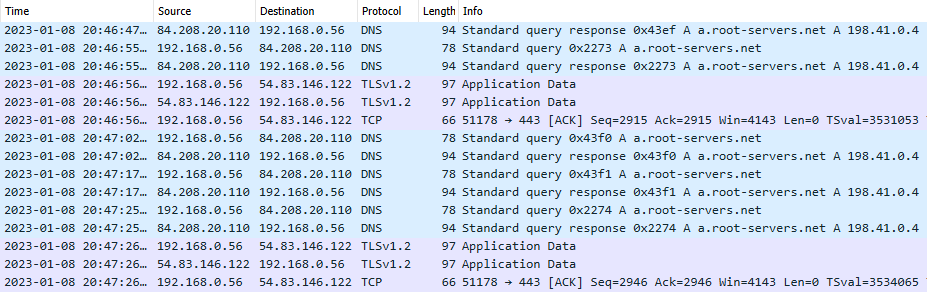
\includegraphics[width=\textwidth]{figures/Wireshark_standby_reoccuring.png}
    \caption{Reoccuring pattern in Standby traffic}
    \label{fig:WSR}
\end{figure}

There is continuous traffic sent towards the configured DNS server requesting A record for a.root-servers.net. According to TP-Link access point this is a mechanism to validate Internet connectivity. If a DNS response with A record it will report as online. This traffic is generated by the TP-Link access point it self and is therefore not relevant for this thesis. 
\begin{itemize}
    \item \textbf{n-devs-gw.tplinkcloud.com}
    \item \textbf{n-deventry-gw.tplinkcloud.com}
\end{itemize}
The IP addresses in the response record can be used in a filter, to remove all traffic not created by the vacuum cleaner. 


If we filter away the DNS traffic there is only application traffic left. As illustrated in figure XX. Since normal smart home devices are behind NAT, the traffic needs to be initiated from the vacuum cleaner it self. Any TCP connections needs to continuously send keep alive packets to keep the communication channel open. Since some of the functionality need s to be initiated from the application via the cloud service. 

\begin{figure}[!ht]
    \centering
    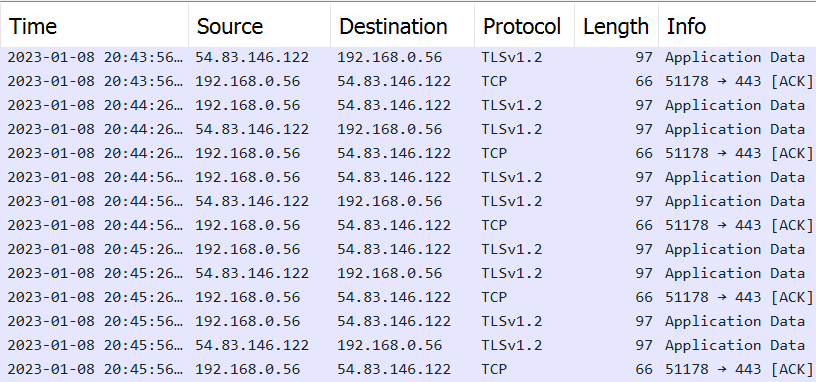
\includegraphics[width=\textwidth]{figures/Wireshark_standby_noDNS.png}
    \caption{Reoccuring pattern application data}
    \label{fig:SBnDNS}
\end{figure}

Figure Keep alive TCP

There is 5 DNS request towards irobot's domain, reoccurring every day. That is: 
\begin{itemize}
    \item \textbf{0.irobot.pool.ntp.org}
    \item \textbf{0.irobot.pool.ntp.org}
    \item \textbf{disc-prod.iot.irobotapi.com}
    \item \textbf{unauth1.prod.iot.irobotapi.com}
    \item \textbf{a2uowfjvhio0fa.iot.us-east-1.amazonaws.com}
\end{itemize}

The continuous TCP keep alive packets are sent to the IP-address in the reply for \textbf{a2uowfjvhio0fa.iot.us-east-1.amazonaws.com}. These IP-addresses and DNS response can be used to identify the correct communication channel used to send commands to the vacuum cleaner. These requests will occure once every day, and the corresponding IP-address will also change, due to DNS load-balancing. 
\chapter{Analysis and Results}
In this chapter the analysis and the result of the research findings will be presented. The overall structure will follow the structure of the chapter Methodology to easier correlate method used and the presented analysis. 

\begin{figure}[H]
    \centering
    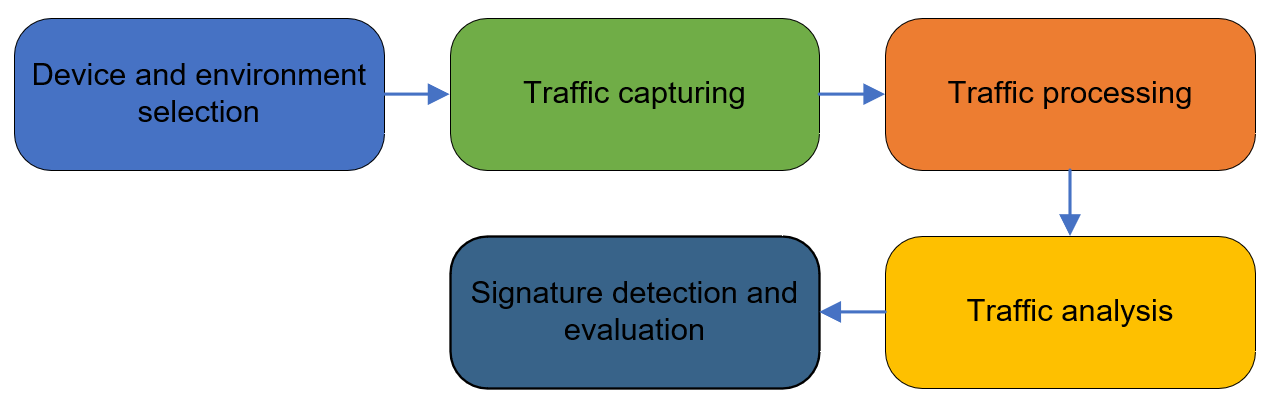
\includegraphics[width=\textwidth]{figures/AnalysisFlow.png}
    \caption{Analysis Flow}
    \label{fig:AnalysisFlow}
\end{figure}

\section{Device and environment selection}
Irobot Roomba i7 was selected as the preferred robot vacuum cleaner in this research, in the corresponding section in chapter Method. In this section the rest of the devices in the smart home environment will be presented. 

\paragraph{Capturing platfrom}
Capturing platform is chosen to be a Raspberry PI 3b+, loaded with Kali Linux operation system. The reason for this is the availability. The author of this thesis had available raspberry PIs through his work. Kali Lunux is open source and have deigned versions to run on Raspberry PI. The OS also includes the analysis tools Wireshark and Tshark that is required in this research. 
An external Wi-Fi adapter is added to the Raspberry PI, this was recommended by \cite{wifi_adapter_monitor_mode}. This also allows data to be extracted from the capturing platform via ftp services on the build in wi-fi network interface card.

\begin{itemize}
    \item wlan0, is buildt in wi-fi interface card
    \item wlan1, is the external TP-LINK TL-WN722N V2 adapter
    \item eth0, is the buldt in ethernet IEEE 802.3 interface card
\end{itemize}

\begin{table}[H]
\centering
\caption{Capturing platform specifications}
\label{tab:CapturingPlatfromSpec}
\begin{tabular}{|ll|}
\hline
\multicolumn{2}{|c|}{\textbf{Capturing platform}}                         \\ \hline
\multicolumn{1}{|l|}{Hardware}               & Raspberry Pi 3b+           \\ \hline
\multicolumn{1}{|l|}{Software}               & Kali Linux                 \\ \hline
\multicolumn{1}{|l|}{Tshark}                 & Version                    \\ \hline
\multicolumn{1}{|l|}{External wi-fi adapter} & TP-LINK TL-WN722N V2       \\ \hline
\multicolumn{1}{|l|}{External storage}       & Micro SD card SanDisk 32GB \\ \hline
\end{tabular}
\end{table}

\paragraph{Analysis platform}
HP Elitebook with windows 11 is used abs the analysis platform, the reason is the availability of the machine. It is installed with Wireshark, Tshark and VS code. 

\begin{table}[H]
\centering
\caption{Analysis platform specifications}
\label{tab:AnalysisPlatfromSpec}
\begin{tabular}{|ll|}
\hline
\multicolumn{2}{|c|}{\textbf{Analysis platform}}      \\ \hline
\multicolumn{1}{|l|}{Hardware}  & HP Elitebook        \\ \hline
\multicolumn{1}{|l|}{Software}  & Windows 11          \\ \hline
\multicolumn{1}{|l|}{Wireshark} & 4.0.2               \\ \hline
\multicolumn{1}{|l|}{VS code}   & 1.77.3 (user setup) \\ \hline
\end{tabular}
\end{table}

\paragraph{Access point}
TP-Link Archer MR200 is acuired, this access point have LAN ports to connect towards the ISP router and wireless capabilities. It can separate connected WLAN and LAN with the use of Network address translation. 

\begin{table}[H]
\centering
\caption{Access point specifications}
\label{tab:AccessPointSpec}
\begin{tabular}{|ll|}
\hline
\multicolumn{2}{|c|}{\textbf{Access Point}}                        \\ \hline
\multicolumn{1}{|l|}{Hardware} & TP-Link archer MR200(EU) ver:5.30 \\ \hline
\multicolumn{1}{|l|}{Software} & version                           \\ \hline
\end{tabular}
\end{table}

\paragraph{LAN Switch}
A Cisco Catalyst 2960 series switch is used, this due to the support for SPAN port configuration. 

\begin{table}[H]
\centering
\caption{LAN Switch specifications}
\label{tab:LanSwitchSpec}
\begin{tabular}{|ll|}
\hline
\multicolumn{2}{|c|}{\textbf{LAN Switch}}                           \\ \hline
\multicolumn{1}{|l|}{Hardware} & Cisco Catalyst 2960 series, 8 port \\ \hline
\multicolumn{1}{|l|}{Software} & ISO 12.2(35)SE5                    \\ \hline
\end{tabular}
\end{table}


\subsection{Smart Home environment}
All these devices connected will create the WLAN/LAN which is used in all environments through this research. The only change will be the Internet delivered by the ISP, if not local configuration and impact is not taken into account this could weekend the reliability of the result. Optimal there would be a completely different smart home infrastructure, but due to limited resources and time it was done with the same internal smart home network. The complete overview is illustrated in \ref{fig:SmartHomeSetup} 

\begin{figure}[H]
    \centering
    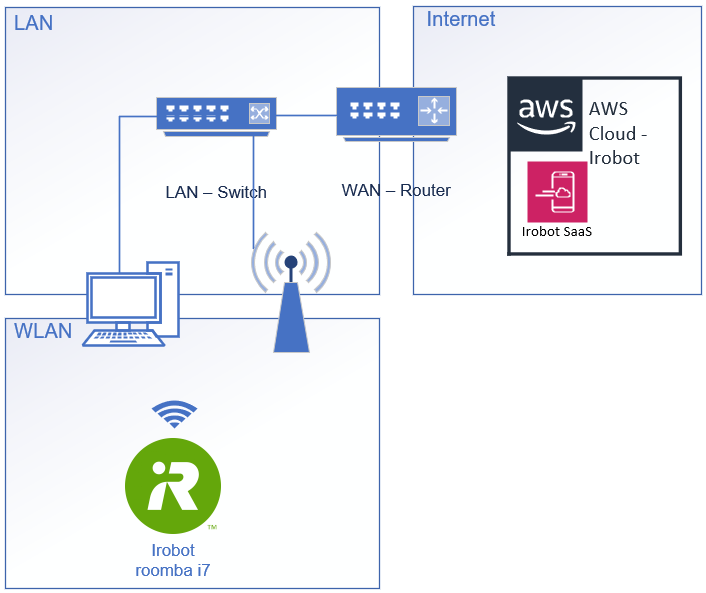
\includegraphics[width=\textwidth]{figures/SmartHomeSetup.png}
    \caption{SmartHomeSetup}
    \label{fig:SmartHomeSetup}
\end{figure}

\section{Traffic Capturing}

\subsection{First test round i Environment 1}
Test matrix for first round in \ref{tab:FirstRoundOfTests}

\begin{table}[H]
\centering
\caption{Test matrix environment 1}
\label{tab:TestMatrixEnv1}
\begin{tabular}{|lllllllllll|}
\hline
\multicolumn{11}{|c|}{\textbf{Scheduled cleaning}}                                                                                                                                                                                                                                                        \\ \hline
\multicolumn{1}{|l|}{Number} & \multicolumn{1}{l|}{1}     & \multicolumn{1}{l|}{2}     & \multicolumn{1}{l|}{3}     & \multicolumn{1}{l|}{4}     & \multicolumn{1}{l|}{5}     & \multicolumn{1}{l|}{6}     & \multicolumn{1}{l|}{7}     & \multicolumn{1}{l|}{8}     & \multicolumn{1}{l|}{9}     & 10    \\ \hline
\multicolumn{1}{|l|}{Date}   & \multicolumn{1}{l|}{10.03} & \multicolumn{1}{l|}{10.03} & \multicolumn{1}{l|}{10.03} & \multicolumn{1}{l|}{10.03} & \multicolumn{1}{l|}{10.03} & \multicolumn{1}{l|}{10.03} & \multicolumn{1}{l|}{10.03} & \multicolumn{1}{l|}{10.03} & \multicolumn{1}{l|}{11.03} & 11.03 \\ \hline
\multicolumn{1}{|l|}{Start}  & \multicolumn{1}{l|}{10:44} & \multicolumn{1}{l|}{11:14} & \multicolumn{1}{l|}{12:14} & \multicolumn{1}{l|}{13:29} & \multicolumn{1}{l|}{14:59} & \multicolumn{1}{l|}{15:29} & \multicolumn{1}{l|}{15:54} & \multicolumn{1}{l|}{16:09} & \multicolumn{1}{l|}{10:09} & 10:29 \\ \hline
\multicolumn{1}{|l|}{End}    & \multicolumn{1}{l|}{10:54} & \multicolumn{1}{l|}{11:24} & \multicolumn{1}{l|}{12:24} & \multicolumn{1}{l|}{13:39} & \multicolumn{1}{l|}{15:09} & \multicolumn{1}{l|}{15:39} & \multicolumn{1}{l|}{16:04} & \multicolumn{1}{l|}{16:19} & \multicolumn{1}{l|}{10:19} & 10:39 \\ \hline
\multicolumn{11}{|c|}{\textbf{Application triggered cleaning}}                                                                                                                                                                                                                                            \\ \hline
\multicolumn{1}{|l|}{Number} & \multicolumn{1}{l|}{1}     & \multicolumn{1}{l|}{2}     & \multicolumn{1}{l|}{3}     & \multicolumn{1}{l|}{4}     & \multicolumn{1}{l|}{5}     & \multicolumn{1}{l|}{6}     & \multicolumn{1}{l|}{7}     & \multicolumn{1}{l|}{8}     & \multicolumn{1}{l|}{9}     & 10    \\ \hline
\multicolumn{1}{|l|}{Date}   & \multicolumn{1}{l|}{28.02} & \multicolumn{1}{l|}{28.02} & \multicolumn{1}{l|}{01.03} & \multicolumn{1}{l|}{09.03} & \multicolumn{1}{l|}{09.03} & \multicolumn{1}{l|}{09.03} & \multicolumn{1}{l|}{09.03} & \multicolumn{1}{l|}{09.03} & \multicolumn{1}{l|}{12.03} & 12.03 \\ \hline
\multicolumn{1}{|l|}{Start}  & \multicolumn{1}{l|}{18:20} & \multicolumn{1}{l|}{18:35} & \multicolumn{1}{l|}{18:53} & \multicolumn{1}{l|}{07:44} & \multicolumn{1}{l|}{08:03} & \multicolumn{1}{l|}{08:25} & \multicolumn{1}{l|}{08:57} & \multicolumn{1}{l|}{09:18} & \multicolumn{1}{l|}{12:20} & 12:54 \\ \hline
\multicolumn{1}{|l|}{End}    & \multicolumn{1}{l|}{18:27} & \multicolumn{1}{l|}{18:42} & \multicolumn{1}{l|}{19:00} & \multicolumn{1}{l|}{07:49} & \multicolumn{1}{l|}{08:10} & \multicolumn{1}{l|}{08:31} & \multicolumn{1}{l|}{09:04} & \multicolumn{1}{l|}{09:26} & \multicolumn{1}{l|}{12:35} & 13:09 \\ \hline
\multicolumn{11}{|c|}{\textbf{Open application}}                                                                                                                                                                                                                                                          \\ \hline
\multicolumn{1}{|l|}{Number} & \multicolumn{1}{l|}{1}     & \multicolumn{1}{l|}{2}     & \multicolumn{1}{l|}{3}     & \multicolumn{1}{l|}{4}     & \multicolumn{1}{l|}{5}     & \multicolumn{1}{l|}{6}     & \multicolumn{1}{l|}{7}     & \multicolumn{1}{l|}{8}     & \multicolumn{1}{l|}{9}     & 10    \\ \hline
\multicolumn{1}{|l|}{Date}   & \multicolumn{1}{l|}{10.03} & \multicolumn{1}{l|}{10.03} & \multicolumn{1}{l|}{10.03} & \multicolumn{1}{l|}{10.03} & \multicolumn{1}{l|}{10.03} & \multicolumn{1}{l|}{10.03} & \multicolumn{1}{l|}{10.03} & \multicolumn{1}{l|}{10.03} & \multicolumn{1}{l|}{11.03} & 11.03 \\ \hline
\multicolumn{1}{|l|}{Start}  & \multicolumn{1}{l|}{10:26} & \multicolumn{1}{l|}{11:06} & \multicolumn{1}{l|}{11:56} & \multicolumn{1}{l|}{13:22} & \multicolumn{1}{l|}{14:58} & \multicolumn{1}{l|}{15:27} & \multicolumn{1}{l|}{15:51} & \multicolumn{1}{l|}{16:07} & \multicolumn{1}{l|}{10:06} & 10:22 \\ \hline
\multicolumn{1}{|l|}{End}    & \multicolumn{1}{l|}{10:36} & \multicolumn{1}{l|}{11:16} & \multicolumn{1}{l|}{12:06} & \multicolumn{1}{l|}{13:32} & \multicolumn{1}{l|}{15:08} & \multicolumn{1}{l|}{15:37} & \multicolumn{1}{l|}{16:01} & \multicolumn{1}{l|}{16:17} & \multicolumn{1}{l|}{10:16} & 10:32 \\ \hline
\multicolumn{11}{|c|}{\textbf{Remove bin}}                                                                                                                                                                                                                                                                \\ \hline
\multicolumn{1}{|l|}{Number} & \multicolumn{1}{l|}{1}     & \multicolumn{1}{l|}{2}     & \multicolumn{1}{l|}{3}     & \multicolumn{1}{l|}{4}     & \multicolumn{1}{l|}{5}     & \multicolumn{1}{l|}{6}     & \multicolumn{1}{l|}{7}     & \multicolumn{1}{l|}{8}     & \multicolumn{1}{l|}{9}     & 10    \\ \hline
\multicolumn{1}{|l|}{Date}   & \multicolumn{1}{l|}{11.03} & \multicolumn{1}{l|}{11.03} & \multicolumn{1}{l|}{11.03} & \multicolumn{1}{l|}{11.03} & \multicolumn{1}{l|}{11.03} & \multicolumn{1}{l|}{11.03} & \multicolumn{1}{l|}{11.03} & \multicolumn{1}{l|}{11.03} & \multicolumn{1}{l|}{11.03} & 11.03 \\ \hline
\multicolumn{1}{|l|}{Start}  & \multicolumn{1}{l|}{17:30} & \multicolumn{1}{l|}{17:35} & \multicolumn{1}{l|}{17:40} & \multicolumn{1}{l|}{17:44} & \multicolumn{1}{l|}{17:47} & \multicolumn{1}{l|}{17:49} & \multicolumn{1}{l|}{17:51} & \multicolumn{1}{l|}{17:53} & \multicolumn{1}{l|}{17:55} & 18:01 \\ \hline
\multicolumn{1}{|l|}{End}    & \multicolumn{1}{l|}{17:31} & \multicolumn{1}{l|}{17:36} & \multicolumn{1}{l|}{17:41} & \multicolumn{1}{l|}{17:45} & \multicolumn{1}{l|}{17:48} & \multicolumn{1}{l|}{17:50} & \multicolumn{1}{l|}{17:52} & \multicolumn{1}{l|}{17:54} & \multicolumn{1}{l|}{17:56} & 18:02 \\ \hline
\multicolumn{11}{|c|}{\textbf{Physical triggered cleaning}}                                                                                                                                                                                                                                               \\ \hline
\multicolumn{1}{|l|}{Number} & \multicolumn{1}{l|}{1}     & \multicolumn{1}{l|}{2}     & \multicolumn{1}{l|}{3}     & \multicolumn{1}{l|}{4}     & \multicolumn{1}{l|}{5}     & \multicolumn{1}{l|}{6}     & \multicolumn{1}{l|}{7}     & \multicolumn{1}{l|}{8}     & \multicolumn{1}{l|}{9}     & 10    \\ \hline
\multicolumn{1}{|l|}{Date}   & \multicolumn{1}{l|}{23.02} & \multicolumn{1}{l|}{23.02} & \multicolumn{1}{l|}{23.02} & \multicolumn{1}{l|}{23.02} & \multicolumn{1}{l|}{23.02} & \multicolumn{1}{l|}{09.03} & \multicolumn{1}{l|}{09.03} & \multicolumn{1}{l|}{09.03} & \multicolumn{1}{l|}{09.03} & 09.03 \\ \hline
\multicolumn{1}{|l|}{Start}  & \multicolumn{1}{l|}{18:08} & \multicolumn{1}{l|}{18:36} & \multicolumn{1}{l|}{19:14} & \multicolumn{1}{l|}{20:13} & \multicolumn{1}{l|}{20:44} & \multicolumn{1}{l|}{09:43} & \multicolumn{1}{l|}{10:30} & \multicolumn{1}{l|}{12:32} & \multicolumn{1}{l|}{13:16} & 17:44 \\ \hline
\multicolumn{1}{|l|}{End}    & \multicolumn{1}{l|}{18:24} & \multicolumn{1}{l|}{19:05} & \multicolumn{1}{l|}{19:34} & \multicolumn{1}{l|}{20:35} & \multicolumn{1}{l|}{21:06} & \multicolumn{1}{l|}{10:02} & \multicolumn{1}{l|}{10:50} & \multicolumn{1}{l|}{12:50} & \multicolumn{1}{l|}{14:05} & 18:05 \\ \hline
\multicolumn{11}{|c|}{\textbf{Automated cleaning}}                                                                                                                                                                                                                                                        \\ \hline
\multicolumn{1}{|l|}{Number} & \multicolumn{1}{l|}{1}     & \multicolumn{1}{l|}{2}     & \multicolumn{1}{l|}{3}     & \multicolumn{1}{l|}{4}     & \multicolumn{1}{l|}{5}     & \multicolumn{1}{l|}{6}     & \multicolumn{1}{l|}{7}     & \multicolumn{1}{l|}{8}     & \multicolumn{1}{l|}{9}     & 10    \\ \hline
\multicolumn{1}{|l|}{Date}   & \multicolumn{1}{l|}{21.02} & \multicolumn{1}{l|}{22.02} & \multicolumn{1}{l|}{23.02} & \multicolumn{1}{l|}{01.03} & \multicolumn{1}{l|}{02.03} & \multicolumn{1}{l|}{03.03} & \multicolumn{1}{l|}{06.03} & \multicolumn{1}{l|}{07.03} & \multicolumn{1}{l|}{08.03} & 09.03 \\ \hline
\multicolumn{1}{|l|}{Start}  & \multicolumn{1}{l|}{21:06} & \multicolumn{1}{l|}{07:37} & \multicolumn{1}{l|}{10:10} & \multicolumn{1}{l|}{07:42} & \multicolumn{1}{l|}{11:05} & \multicolumn{1}{l|}{07:03} & \multicolumn{1}{l|}{07:04} & \multicolumn{1}{l|}{08:42} & \multicolumn{1}{l|}{07:49} & 07:22 \\ \hline
\multicolumn{1}{|l|}{End}    & \multicolumn{1}{l|}{21:14} & \multicolumn{1}{l|}{07:45} & \multicolumn{1}{l|}{10:16} & \multicolumn{1}{l|}{07:47} & \multicolumn{1}{l|}{11:10} & \multicolumn{1}{l|}{07:08} & \multicolumn{1}{l|}{07:09} & \multicolumn{1}{l|}{08:47} & \multicolumn{1}{l|}{07:54} & 07:29 \\ \hline
\end{tabular}
\end{table}

\begin{table}[H]
\centering
\caption{Test matrix environment 2}
\label{tab:TestMatrixEnv2}
\begin{tabular}{|lllllllllll|}
\hline
\multicolumn{11}{|c|}{\textbf{Scheduled cleaning}}                                                                                                                                                                                                                                                        \\ \hline
\multicolumn{1}{|l|}{Number} & \multicolumn{1}{l|}{1}     & \multicolumn{1}{l|}{2}     & \multicolumn{1}{l|}{3}     & \multicolumn{1}{l|}{4}     & \multicolumn{1}{l|}{5}     & \multicolumn{1}{l|}{6}     & \multicolumn{1}{l|}{7}     & \multicolumn{1}{l|}{8}     & \multicolumn{1}{l|}{9}     & 10    \\ \hline
\multicolumn{1}{|l|}{Date}   & \multicolumn{1}{l|}{25.02} & \multicolumn{1}{l|}{25.02} & \multicolumn{1}{l|}{26.02} & \multicolumn{1}{l|}{26.02} & \multicolumn{1}{l|}{26.02} & \multicolumn{1}{l|}{26.02} & \multicolumn{1}{l|}{26.02} & \multicolumn{1}{l|}{26.02} & \multicolumn{1}{l|}{26.02} & 26.02 \\ \hline
\multicolumn{1}{|l|}{Start}  & \multicolumn{1}{l|}{20:30} & \multicolumn{1}{l|}{21:00} & \multicolumn{1}{l|}{11:20} & \multicolumn{1}{l|}{11:50} & \multicolumn{1}{l|}{12:20} & \multicolumn{1}{l|}{12:50} & \multicolumn{1}{l|}{13:20} & \multicolumn{1}{l|}{13:50} & \multicolumn{1}{l|}{14:20} & 15:00 \\ \hline
\multicolumn{1}{|l|}{End}    & \multicolumn{1}{l|}{20:45} & \multicolumn{1}{l|}{21:15} & \multicolumn{1}{l|}{11:35} & \multicolumn{1}{l|}{12:05} & \multicolumn{1}{l|}{12:35} & \multicolumn{1}{l|}{13:05} & \multicolumn{1}{l|}{13:35} & \multicolumn{1}{l|}{14:05} & \multicolumn{1}{l|}{14:35} & 15:15 \\ \hline
\multicolumn{11}{|c|}{\textbf{Application triggered cleaning}}                                                                                                                                                                                                                                            \\ \hline
\multicolumn{1}{|l|}{Number} & \multicolumn{1}{l|}{1}     & \multicolumn{1}{l|}{2}     & \multicolumn{1}{l|}{3}     & \multicolumn{1}{l|}{4}     & \multicolumn{1}{l|}{5}     & \multicolumn{1}{l|}{6}     & \multicolumn{1}{l|}{7}     & \multicolumn{1}{l|}{8}     & \multicolumn{1}{l|}{9}     & 10    \\ \hline
\multicolumn{1}{|l|}{Date}   & \multicolumn{1}{l|}{25.02} & \multicolumn{1}{l|}{25.02} & \multicolumn{1}{l|}{25.02} & \multicolumn{1}{l|}{25.02} & \multicolumn{1}{l|}{25.02} & \multicolumn{1}{l|}{25.02} & \multicolumn{1}{l|}{25.02} & \multicolumn{1}{l|}{25.02} & \multicolumn{1}{l|}{25.02} & 25.02 \\ \hline
\multicolumn{1}{|l|}{Start}  & \multicolumn{1}{l|}{14:30} & \multicolumn{1}{l|}{15:00} & \multicolumn{1}{l|}{15:30} & \multicolumn{1}{l|}{16:00} & \multicolumn{1}{l|}{16:30} & \multicolumn{1}{l|}{17:00} & \multicolumn{1}{l|}{17:30} & \multicolumn{1}{l|}{19:00} & \multicolumn{1}{l|}{19:30} & 20:00 \\ \hline
\multicolumn{1}{|l|}{End}    & \multicolumn{1}{l|}{14:45} & \multicolumn{1}{l|}{15:15} & \multicolumn{1}{l|}{15:45} & \multicolumn{1}{l|}{16:15} & \multicolumn{1}{l|}{16:45} & \multicolumn{1}{l|}{17:15} & \multicolumn{1}{l|}{17:45} & \multicolumn{1}{l|}{19:15} & \multicolumn{1}{l|}{19:45} & 20:15 \\ \hline
\multicolumn{11}{|c|}{\textbf{Open application}}                                                                                                                                                                                                                                                          \\ \hline
\multicolumn{1}{|l|}{Number} & \multicolumn{1}{l|}{1}     & \multicolumn{1}{l|}{2}     & \multicolumn{1}{l|}{3}     & \multicolumn{1}{l|}{4}     & \multicolumn{1}{l|}{5}     & \multicolumn{1}{l|}{6}     & \multicolumn{1}{l|}{7}     & \multicolumn{1}{l|}{8}     & \multicolumn{1}{l|}{9}     & 10    \\ \hline
\multicolumn{1}{|l|}{Date}   & \multicolumn{1}{l|}{25.02} & \multicolumn{1}{l|}{25.02} & \multicolumn{1}{l|}{25.02} & \multicolumn{1}{l|}{25.02} & \multicolumn{1}{l|}{26.02} & \multicolumn{1}{l|}{26.02} & \multicolumn{1}{l|}{26.02} & \multicolumn{1}{l|}{26.02} & \multicolumn{1}{l|}{26.02} & 26.02 \\ \hline
\multicolumn{1}{|l|}{Start}  & \multicolumn{1}{l|}{20:50} & \multicolumn{1}{l|}{21:20} & \multicolumn{1}{l|}{22:20} & \multicolumn{1}{l|}{22:50} & \multicolumn{1}{l|}{11:10} & \multicolumn{1}{l|}{11:40} & \multicolumn{1}{l|}{12:10} & \multicolumn{1}{l|}{12:40} & \multicolumn{1}{l|}{13:10} & 13:40 \\ \hline
\multicolumn{1}{|l|}{End}    & \multicolumn{1}{l|}{20:52} & \multicolumn{1}{l|}{21:21} & \multicolumn{1}{l|}{22:22} & \multicolumn{1}{l|}{22:52} & \multicolumn{1}{l|}{11:11} & \multicolumn{1}{l|}{11:41} & \multicolumn{1}{l|}{12:11} & \multicolumn{1}{l|}{12:41} & \multicolumn{1}{l|}{13:11} & 13:41 \\ \hline
\multicolumn{11}{|c|}{\textbf{Remove bin}}                                                                                                                                                                                                                                                                \\ \hline
\multicolumn{1}{|l|}{Number} & \multicolumn{1}{l|}{1}     & \multicolumn{1}{l|}{2}     & \multicolumn{1}{l|}{3}     & \multicolumn{1}{l|}{4}     & \multicolumn{1}{l|}{5}     & \multicolumn{1}{l|}{6}     & \multicolumn{1}{l|}{7}     & \multicolumn{1}{l|}{8}     & \multicolumn{1}{l|}{9}     & 10    \\ \hline
\multicolumn{1}{|l|}{Date}   & \multicolumn{1}{l|}{26.02} & \multicolumn{1}{l|}{26.02} & \multicolumn{1}{l|}{26.02} & \multicolumn{1}{l|}{27.02} & \multicolumn{1}{l|}{27.02} & \multicolumn{1}{l|}{27.02} & \multicolumn{1}{l|}{27.02} & \multicolumn{1}{l|}{27.02} & \multicolumn{1}{l|}{27.02} & 27.02 \\ \hline
\multicolumn{1}{|l|}{Start}  & \multicolumn{1}{l|}{15:22} & \multicolumn{1}{l|}{15:30} & \multicolumn{1}{l|}{15:35} & \multicolumn{1}{l|}{15:05} & \multicolumn{1}{l|}{15:10} & \multicolumn{1}{l|}{15:15} & \multicolumn{1}{l|}{15:20} & \multicolumn{1}{l|}{15:25} & \multicolumn{1}{l|}{15:30} & 15:35 \\ \hline
\multicolumn{1}{|l|}{End}    & \multicolumn{1}{l|}{15:23} & \multicolumn{1}{l|}{15:31} & \multicolumn{1}{l|}{15:36} & \multicolumn{1}{l|}{15:06} & \multicolumn{1}{l|}{15:11} & \multicolumn{1}{l|}{15:16} & \multicolumn{1}{l|}{15:21} & \multicolumn{1}{l|}{15:26} & \multicolumn{1}{l|}{15:31} & 15:36 \\ \hline
\multicolumn{11}{|c|}{\textbf{Physical triggered cleaning}}                                                                                                                                                                                                                                               \\ \hline
\multicolumn{1}{|l|}{Number} & \multicolumn{1}{l|}{1}     & \multicolumn{1}{l|}{2}     & \multicolumn{1}{l|}{3}     & \multicolumn{1}{l|}{4}     & \multicolumn{1}{l|}{5}     & \multicolumn{1}{l|}{6}     & \multicolumn{1}{l|}{7}     & \multicolumn{1}{l|}{8}     & \multicolumn{1}{l|}{9}     & 10    \\ \hline
\multicolumn{1}{|l|}{Date}   & \multicolumn{1}{l|}{25.02} & \multicolumn{1}{l|}{25.02} & \multicolumn{1}{l|}{25.02} & \multicolumn{1}{l|}{25.02} & \multicolumn{1}{l|}{25.02} & \multicolumn{1}{l|}{26.02} & \multicolumn{1}{l|}{26.02} & \multicolumn{1}{l|}{26.02} & \multicolumn{1}{l|}{26.02} & 26.02 \\ \hline
\multicolumn{1}{|l|}{Start}  & \multicolumn{1}{l|}{22:00} & \multicolumn{1}{l|}{22:30} & \multicolumn{1}{l|}{23:00} & \multicolumn{1}{l|}{23:20} & \multicolumn{1}{l|}{23:40} & \multicolumn{1}{l|}{00:00} & \multicolumn{1}{l|}{00:20} & \multicolumn{1}{l|}{00:40} & \multicolumn{1}{l|}{01:06} & 01:31 \\ \hline
\multicolumn{1}{|l|}{End}    & \multicolumn{1}{l|}{22:12} & \multicolumn{1}{l|}{22:45} & \multicolumn{1}{l|}{23:15} & \multicolumn{1}{l|}{23:35} & \multicolumn{1}{l|}{23:55} & \multicolumn{1}{l|}{00:15} & \multicolumn{1}{l|}{00:35} & \multicolumn{1}{l|}{00:55} & \multicolumn{1}{l|}{01:20} & 01:45 \\ \hline
\multicolumn{11}{|c|}{\textbf{Automated cleaning}}                                                                                                                                                                                                                                                        \\ \hline
\multicolumn{1}{|l|}{Number} & \multicolumn{1}{l|}{1}     & \multicolumn{1}{l|}{2}     & \multicolumn{1}{l|}{3}     & \multicolumn{1}{l|}{4}     & \multicolumn{1}{l|}{5}     & \multicolumn{1}{l|}{6}     & \multicolumn{1}{l|}{7}     & \multicolumn{1}{l|}{8}     & \multicolumn{1}{l|}{9}     & 10    \\ \hline
\multicolumn{1}{|l|}{Date}   & \multicolumn{1}{l|}{25.02} & \multicolumn{1}{l|}{26.02} & \multicolumn{1}{l|}{26.02} & \multicolumn{1}{l|}{26.02} & \multicolumn{1}{l|}{26.02} & \multicolumn{1}{l|}{27.02} & \multicolumn{1}{l|}{27.02} & \multicolumn{1}{l|}{27.02} & \multicolumn{1}{l|}{27.02} & 27.02 \\ \hline
\multicolumn{1}{|l|}{Start}  & \multicolumn{1}{l|}{21:32} & \multicolumn{1}{l|}{01:53} & \multicolumn{1}{l|}{15:43} & \multicolumn{1}{l|}{17:00} & \multicolumn{1}{l|}{22:11} & \multicolumn{1}{l|}{07:57} & \multicolumn{1}{l|}{08:51} & \multicolumn{1}{l|}{11:03} & \multicolumn{1}{l|}{12:04} & 13:36 \\ \hline
\multicolumn{1}{|l|}{End}    & \multicolumn{1}{l|}{21:50} & \multicolumn{1}{l|}{02:10} & \multicolumn{1}{l|}{15:55} & \multicolumn{1}{l|}{17:12} & \multicolumn{1}{l|}{22:23} & \multicolumn{1}{l|}{08:10} & \multicolumn{1}{l|}{09:02} & \multicolumn{1}{l|}{11:13} & \multicolumn{1}{l|}{12:16} & 13:48 \\ \hline
\end{tabular}
\end{table}
\chapter*{Results}

\section{Test case result}

\subsection{Test 1}

\subsection{Test 2}

\subsection{Test 3}

\section{Result Summary}

\subsection{Countermeasures Suggestion}


\chapter*{Discussion}
\chapter*{Conclusion}

\section{Conclusion}

\section{Future Work}




\chapter*{\bibname}
\printbibliography[heading=none]

%\input{chapters/papers.tex}

%\appendix
%\input{appendices/a-appendix.tex}

\end{document}
